\documentclass[
  jou,
  floatsintext,
  longtable,
  nolmodern,
  notxfonts,
  notimes,
  colorlinks=true,linkcolor=blue,citecolor=blue,urlcolor=blue]{apa7}

\usepackage{amsmath}
\usepackage{amssymb}




\RequirePackage{longtable}
\RequirePackage{threeparttablex}

\makeatletter
\renewcommand{\paragraph}{\@startsection{paragraph}{4}{\parindent}%
	{0\baselineskip \@plus 0.2ex \@minus 0.2ex}%
	{-.5em}%
	{\normalfont\normalsize\bfseries\typesectitle}}

\renewcommand{\subparagraph}[1]{\@startsection{subparagraph}{5}{0.5em}%
	{0\baselineskip \@plus 0.2ex \@minus 0.2ex}%
	{-\z@\relax}%
	{\normalfont\normalsize\bfseries\itshape\hspace{\parindent}{#1}\textit{\addperi}}{\relax}}
\makeatother




\usepackage{longtable, booktabs, multirow, multicol, colortbl, hhline, caption, array, float, xpatch}
\usepackage{subcaption}


\renewcommand\thesubfigure{\Alph{subfigure}}
\setcounter{topnumber}{2}
\setcounter{bottomnumber}{2}
\setcounter{totalnumber}{4}
\renewcommand{\topfraction}{0.85}
\renewcommand{\bottomfraction}{0.85}
\renewcommand{\textfraction}{0.15}
\renewcommand{\floatpagefraction}{0.7}

\usepackage{tcolorbox}
\tcbuselibrary{listings,theorems, breakable, skins}
\usepackage{fontawesome5}

\definecolor{quarto-callout-color}{HTML}{909090}
\definecolor{quarto-callout-note-color}{HTML}{0758E5}
\definecolor{quarto-callout-important-color}{HTML}{CC1914}
\definecolor{quarto-callout-warning-color}{HTML}{EB9113}
\definecolor{quarto-callout-tip-color}{HTML}{00A047}
\definecolor{quarto-callout-caution-color}{HTML}{FC5300}
\definecolor{quarto-callout-color-frame}{HTML}{ACACAC}
\definecolor{quarto-callout-note-color-frame}{HTML}{4582EC}
\definecolor{quarto-callout-important-color-frame}{HTML}{D9534F}
\definecolor{quarto-callout-warning-color-frame}{HTML}{F0AD4E}
\definecolor{quarto-callout-tip-color-frame}{HTML}{02B875}
\definecolor{quarto-callout-caution-color-frame}{HTML}{FD7E14}

%\newlength\Oldarrayrulewidth
%\newlength\Oldtabcolsep


\usepackage{hyperref}




\providecommand{\tightlist}{%
  \setlength{\itemsep}{0pt}\setlength{\parskip}{0pt}}
\usepackage{longtable,booktabs,array}
\usepackage{calc} % for calculating minipage widths
% Correct order of tables after \paragraph or \subparagraph
\usepackage{etoolbox}
\makeatletter
\patchcmd\longtable{\par}{\if@noskipsec\mbox{}\fi\par}{}{}
\makeatother
% Allow footnotes in longtable head/foot
\IfFileExists{footnotehyper.sty}{\usepackage{footnotehyper}}{\usepackage{footnote}}
\makesavenoteenv{longtable}

\usepackage{graphicx}
\makeatletter
\newsavebox\pandoc@box
\newcommand*\pandocbounded[1]{% scales image to fit in text height/width
  \sbox\pandoc@box{#1}%
  \Gscale@div\@tempa{\textheight}{\dimexpr\ht\pandoc@box+\dp\pandoc@box\relax}%
  \Gscale@div\@tempb{\linewidth}{\wd\pandoc@box}%
  \ifdim\@tempb\p@<\@tempa\p@\let\@tempa\@tempb\fi% select the smaller of both
  \ifdim\@tempa\p@<\p@\scalebox{\@tempa}{\usebox\pandoc@box}%
  \else\usebox{\pandoc@box}%
  \fi%
}
% Set default figure placement to htbp
\def\fps@figure{htbp}
\makeatother


% definitions for citeproc citations
\NewDocumentCommand\citeproctext{}{}
\NewDocumentCommand\citeproc{mm}{%
  \begingroup\def\citeproctext{#2}\cite{#1}\endgroup}
\makeatletter
 % allow citations to break across lines
 \let\@cite@ofmt\@firstofone
 % avoid brackets around text for \cite:
 \def\@biblabel#1{}
 \def\@cite#1#2{{#1\if@tempswa , #2\fi}}
\makeatother
\newlength{\cslhangindent}
\setlength{\cslhangindent}{1.5em}
\newlength{\csllabelwidth}
\setlength{\csllabelwidth}{3em}
\newenvironment{CSLReferences}[2] % #1 hanging-indent, #2 entry-spacing
 {\begin{list}{}{%
  \setlength{\itemindent}{0pt}
  \setlength{\leftmargin}{0pt}
  \setlength{\parsep}{0pt}
  % turn on hanging indent if param 1 is 1
  \ifodd #1
   \setlength{\leftmargin}{\cslhangindent}
   \setlength{\itemindent}{-1\cslhangindent}
  \fi
  % set entry spacing
  \setlength{\itemsep}{#2\baselineskip}}}
 {\end{list}}
\usepackage{calc}
\newcommand{\CSLBlock}[1]{\hfill\break\parbox[t]{\linewidth}{\strut\ignorespaces#1\strut}}
\newcommand{\CSLLeftMargin}[1]{\parbox[t]{\csllabelwidth}{\strut#1\strut}}
\newcommand{\CSLRightInline}[1]{\parbox[t]{\linewidth - \csllabelwidth}{\strut#1\strut}}
\newcommand{\CSLIndent}[1]{\hspace{\cslhangindent}#1}





\usepackage{newtx}

\defaultfontfeatures{Scale=MatchLowercase}
\defaultfontfeatures[\rmfamily]{Ligatures=TeX,Scale=1}





\title{\textbf{The Mint Scale: A Fresh Validation of the Multimodal
Interoception Questionnaire and Comparison to the MAIA, BPQ and IAS}}


\shorttitle{Mint Validation}


\usepackage{etoolbox}









\authorsnames[{1,2},{1},{1},{1},{1}]{Dominique Makowski,Ana Neves,Emma
Benn,Maisie Bennett,Giulia Poreiro}







\authorsaffiliations{
{School of Psychology, University of Sussex},{Sussex Centre for
Consciousness Science, University of Sussex}}




\leftheader{Makowski, Neves, Benn, Bennett and Poreiro}



\abstract{Interoception, the sensing of the body's internal state, is an
important component of homeostatic and allostatic regulation with
wide-ranging implications for mental and physical health, yet its
measurement is hindered by tools with conceptual and psychometric
issues. To address these limitations, we developed and validated the
Multimodal Interoception Questionnaire (Mint). In Study 1 (N=559), a
comprehensive item pool using a novel ``modality-by-context'' framework
was generated and then reduced using psychometric network analysis. In
Study 2 (N=737), we validated the Mint in an independent sample,
establishing its structure, comparing its predictive power against
established interoception questionnaires (MAIA-2, BPQ, IAS), and across
a wide range of clinical and cognitive outcomes. This rigorous process
yielded a 33-item scale with a stable hierarchical structure comprising
three metaclusters (Interoceptive Deficit, Interoceptive Awareness,
Visceroception) and 11 distinct facets. The Mint demonstrated superior
criterion validity, consistently outperforming existing scales in
predicting outcomes tied to altered bodily perception, including
alexithymia, ADHD, autism, and somatic symptom clusters. The Mint offers
a psychometrically robust and nuanced measure of self-reported
interoception that integrates and extends existing scales, providing
researchers and clinicians with a practical and readily usable tool to
investigate the role of bodily sensations in health and disease. }

\keywords{Interoception questionnaire, interoceptive accuracy scale,
MAIA, Mint Validation, Body Awareness, Health}

\authornote{\par{\addORCIDlink{Dominique
Makowski}{0000-0001-5375-9967}}\par{\addORCIDlink{Ana
Neves}{0009-0006-0020-7599}}\par{\addORCIDlink{Giulia
Poreiro}{0000-0002-2343-5109}} 
\par{ }
\par{     \begin{tcolorbox}[enhanced jigsaw, colframe=quarto-callout-note-color-frame, rightrule=.15mm, colback=white, toprule=.15mm, breakable, left=2mm, opacityback=0, leftrule=.75mm, bottomrule=.15mm, arc=.35mm]

This preprint is a non-peer-reviewed work from the
\href{https://realitybending.github.io/}{\textbf{Reality Bending Lab}}.

\includegraphics[width=0.2\linewidth,height=\textheight,keepaspectratio]{manuscript_files/mediabag/ReBeL_LogoOnly_hu114.png}

\end{tcolorbox}  Author roles were classified using the Contributor Role
Taxonomy (CRediT; https://credit.niso.org/) as follows:  Dominique
Makowski:   Conceptualization, Data curation, Formal Analysis, Funding
acquisition, Investigation, Methodology, Project
administration, Resources, Software, Supervision, Validation, Visualization, Writing
-- original draft; Ana Neves:   Investigation, Methodology, Project
administration, Supervision, Writing -- original draft, Writing --
review \& editing; Emma Benn:   Investigation; Maisie
Bennett:   Investigation; Giulia
Poreiro:   Investigation, Methodology, Writing -- original
draft, Writing -- review \& editing}
\par{Correspondence concerning this article should be addressed
to Dominique
Makowski, Email: \href{mailto:D.Makowski@sussex.ac.uk}{D.Makowski@sussex.ac.uk}}
}

\usepackage{pbalance}
% \usepackage{float}
\makeatletter
\let\oldtpt\ThreePartTable
\let\endoldtpt\endThreePartTable
\def\ThreePartTable{\@ifnextchar[\ThreePartTable@i \ThreePartTable@ii}
\def\ThreePartTable@i[#1]{\begin{figure}[!htbp]
\onecolumn
\begin{minipage}{0.485\textwidth}
\oldtpt[#1]
}
\def\ThreePartTable@ii{\begin{figure}[!htbp]
\onecolumn
\begin{minipage}{0.48\textwidth}
\oldtpt
}
\def\endThreePartTable{
\endoldtpt
\end{minipage}
\twocolumn
\end{figure}}
\makeatother


\makeatletter
\let\endoldlt\endlongtable		
\def\endlongtable{
\hline
\endoldlt}
\makeatother

\newenvironment{twocolumntable}% environment name
{% begin code
\begin{table*}[!htbp]%
\onecolumn%
}%
{%
\twocolumn%
\end{table*}%
}% end code

\urlstyle{same}



\makeatletter
\@ifpackageloaded{tcolorbox}{}{\usepackage[skins,breakable]{tcolorbox}}
\@ifpackageloaded{fontawesome5}{}{\usepackage{fontawesome5}}
\definecolor{quarto-callout-color}{HTML}{909090}
\definecolor{quarto-callout-note-color}{HTML}{0758E5}
\definecolor{quarto-callout-important-color}{HTML}{CC1914}
\definecolor{quarto-callout-warning-color}{HTML}{EB9113}
\definecolor{quarto-callout-tip-color}{HTML}{00A047}
\definecolor{quarto-callout-caution-color}{HTML}{FC5300}
\definecolor{quarto-callout-color-frame}{HTML}{acacac}
\definecolor{quarto-callout-note-color-frame}{HTML}{4582ec}
\definecolor{quarto-callout-important-color-frame}{HTML}{d9534f}
\definecolor{quarto-callout-warning-color-frame}{HTML}{f0ad4e}
\definecolor{quarto-callout-tip-color-frame}{HTML}{02b875}
\definecolor{quarto-callout-caution-color-frame}{HTML}{fd7e14}
\makeatother
\makeatletter
\@ifpackageloaded{caption}{}{\usepackage{caption}}
\AtBeginDocument{%
\ifdefined\contentsname
  \renewcommand*\contentsname{Table of contents}
\else
  \newcommand\contentsname{Table of contents}
\fi
\ifdefined\listfigurename
  \renewcommand*\listfigurename{List of Figures}
\else
  \newcommand\listfigurename{List of Figures}
\fi
\ifdefined\listtablename
  \renewcommand*\listtablename{List of Tables}
\else
  \newcommand\listtablename{List of Tables}
\fi
\ifdefined\figurename
  \renewcommand*\figurename{Figure}
\else
  \newcommand\figurename{Figure}
\fi
\ifdefined\tablename
  \renewcommand*\tablename{Table}
\else
  \newcommand\tablename{Table}
\fi
}
\@ifpackageloaded{float}{}{\usepackage{float}}
\floatstyle{ruled}
\@ifundefined{c@chapter}{\newfloat{codelisting}{h}{lop}}{\newfloat{codelisting}{h}{lop}[chapter]}
\floatname{codelisting}{Listing}
\newcommand*\listoflistings{\listof{codelisting}{List of Listings}}
\makeatother
\makeatletter
\makeatother
\makeatletter
\@ifpackageloaded{caption}{}{\usepackage{caption}}
\@ifpackageloaded{subcaption}{}{\usepackage{subcaption}}
\makeatother

% From https://tex.stackexchange.com/a/645996/211326
%%% apa7 doesn't want to add appendix section titles in the toc
%%% let's make it do it
\makeatletter
\xpatchcmd{\appendix}
  {\par}
  {\addcontentsline{toc}{section}{\@currentlabelname}\par}
  {}{}
\makeatother

%% Disable longtable counter
%% https://tex.stackexchange.com/a/248395/211326

\usepackage{etoolbox}

\makeatletter
\patchcmd{\LT@caption}
  {\bgroup}
  {\bgroup\global\LTpatch@captiontrue}
  {}{}
\patchcmd{\longtable}
  {\par}
  {\par\global\LTpatch@captionfalse}
  {}{}
\apptocmd{\endlongtable}
  {\ifLTpatch@caption\else\addtocounter{table}{-1}\fi}
  {}{}
\newif\ifLTpatch@caption
\makeatother

\begin{document}

\maketitle



\setcounter{secnumdepth}{-\maxdimen} % remove section numbering

\setlength\LTleft{0pt}




\section{Introduction}\label{introduction}

Interoception - the sensing and interpretation of the body's internal
physiological signals - plays a fundamental role in processes ranging
from homeostatic regulation to emotion, decision-making, and mental
health (\citeproc{ref-craig2002how}{Craig, 2002};
\citeproc{ref-critchley2017interoception}{Critchley \& Garfinkel,
2017}). Despite its growing recognition, the field has been hindered by
inconsistent definitions and fragmented measurement approaches
(\citeproc{ref-desmedt2022measures}{Desmedt et al., 2022},
\citeproc{ref-desmedt2025discrepancies}{2025};
\citeproc{ref-khalsa2018interoception}{Khalsa et al., 2018}). Available
tools include ``objective'' physiological tasks (e.g., heartbeat
counting or tracking) and ``subjective'' self-reports, and encompass
both ``explicit'' paradigms that direct participants' attention to
internal sensations and ``implicit'' paradigms that do not (e.g.,
heartbeat evoked potentials recorded during rest). These assessments are
often targeted at only one of several interoceptive modalities (e.g.,
cardioception, respiroception, gastroception), and are mapped onto
theoretical dimensions (e.g., accuracy, sensitivity, awareness,
\citeproc{ref-garfinkel2015knowing}{Garfinkel et al., 2015}) within a
rapidly evolving theoretical landscape. However, no consensus exists on
a gold-standard measure with each approach having distinct limitations.
For example, physiological tasks often require specialised equipment and
expertise, are time-consuming, and are challenging to administer at
scale, whereas questionnaires are constrained by their inherent
subjectivity. Crucially, the psychometric quality of many of these
measures is questionable (e.g., see criticism about the heartbeat
counting task, \citeproc{ref-zamariola2018interoceptive}{Zamariola et
al., 2018}), yielding low inter-task correlations
(\citeproc{ref-murphy2018classifying}{Murphy et al., 2018}) and raising
important concerns regarding their reliability and validity (e.g.,
measures presented as measuring one theoretical dimension but likely
measuring something else). This lack of conceptual clarity and
measurement convergence impedes scientific progress in comparing,
replicating, and interpreting interoception-related findings,
emphasising the need to develop improved tools that align with modern
psychometric standards.

The present work focuses on self-report questionnaires, which offer a
scalable and accessible tool complementing physiological tasks. Among
the numerous interoceptive questionnaires available, a handful dominate
the literature (\citeproc{ref-desmedt2022measures}{Desmedt et al.,
2022}), including the Body Perception Questionnaire (BPQ,
\citeproc{ref-kolacz2018body}{Kolacz et al., 2018}), the
Multidimensional Assessment of Interoceptive Awareness (MAIA,
\citeproc{ref-mehling2018multidimensional}{Mehling et al., 2018}), and
the Interoceptive Accuracy Scale (IAS,
\citeproc{ref-murphy2018classifying}{Murphy et al., 2018}). These tools
were developed in different eras of a rapidly evolving field, each with
its own objectives and philosophies. For example, the BPQ, one of the
earliest measures, captures bodily awareness and autonomic nervous
system (ANS) reactivity by focusing on experiences of physiological
stress reactions in organs innervated by the ANS, such as those
triggered by stress or trauma (\citeproc{ref-kolacz2018body}{Kolacz et
al., 2018}). The MAIA incorporated ideas from the then-booming emotion
regulation and mindfulness fields, including subscales assessing
adaptive coping strategies and metacognitive insights about the body. In
contrast, the IAS was recently developed to circumvent these high-level
- possibly tangential - constructs, instead capturing subjective reports
of concrete bodily events (e.g., coughing, sneezing) as proxies for
interoceptive accuracy.

These differing philosophies have practical consequences, leading to
poor convergence between scales that are assumed to measure the same
construct (\citeproc{ref-vig2022questionnaires}{Vig et al., 2022}) - a
classic example of the ``jingle fallacy'' where the shared label of
``interoception'' can mask underlying measurand differences, hindering
replication and theoretical integration. In acknowledgement of this
issue, efforts have been made to align subjective measures with
theoretical models that outline different facets of interoception (e.g.,
accuracy, attention, deficits). However, focusing on developing measures
that are theory-driven may however be premature when theoretical models
are in flux, and when a topographic mapping to self-report dimensions is
not guaranteed. For example, interoceptive distinctions that are
relevant at a neuroanatomical or cognitive level might not necessarily
map onto the structure of subjective experiences. More fundamentally,
existing interoception questionnaires typically fail to consider the
full range of interoceptive modalities and the context in which
interoceptive experiences occur. Most existing questionnaires focus on a
narrow range of bodily modalities, with a heavy bias towards
cardio-respiratory sensations at the expense of others like gastric,
urogenital, or thermoregulatory signals.

Perhaps most critically, existing measures often ask participants to
make general assessments across most/all contexts, which does not
capture the potential homeostatic relevance of attending or detecting
internal signals. For example, the BPQ asks participants to reflect on
how often during most situations a person is aware of various bodily
sensations, such as their heart beating. Without a contextual reference
point, there is likely to be substantial variability in how participants
interpret and respond to items as well as what those responses might
mean about their interoceptive abilities. A general item about ``feeling
your heart beat'' is ambiguous since its salience, frequency, experience
and interpretation would differ depending on the context, which may or
may not be relevant homeostatically. For instance, awareness of one's
heartbeat may occur across multiple contexts, including during physical
exercise, a moment of anxiety, excitement, or quiet rest with awareness
across different contexts reflecting something different about
interoceptive sensations. This is further complicated by retrospective
memory biases such that individuals respond with the most easily
accessible or recent instances of awareness; for example, someone who
exercises regularly, or is anxious, might more easily recall an instance
of occurrence of feeling their heart beating and respond based on that
contextual saliency. As an exception, the MAIA does provide some
contextual cues for participants (e.g., ``When something is wrong in my
life I can feel it in my body'') but this is inconsistent across items
and focuses almost exclusively on negative (e.g., painful) and emotional
(e.g., angry, joyful) contexts as well as general `body' sensations
rather than specific interoceptive modalities. Thus, no existing scale
captures subjective assessments across multiple interoceptive modalities
and across different contexts in which interoceptive experiences occur.

To address this gap, we developed and validated the Multimodal
Interoception Questionnaire (Mint), a new questionnaire that
systematically addresses the above limitations. In Study 1, we describe
the bottom-up development of the Mint, using a ``modality-by-context''
framework to generate a comprehensive item pool, which was then refined
using cutting-edge psychometric network analysis. In Study 2, we
validated the final 33-item version of the Mint against the established
interoception questionnaires, demonstrating its robust structure and
predictive validity for a range of clinically-relevant outcomes.

\section{Study 1: Item Selection}\label{study-1-item-selection}

The aim of Study 1 was to develop a new interoception questionnaire by
generating a comprehensive item pool and subsequently refining it into a
psychometrically robust scale. To overcome the limitations of existing
questionnaires, we adopted a bottom-up, theoretically agnostic approach.
Rather than imposing a pre-defined theoretical structure on
questionnaire items, we instead focused on two tangible and
systematically controllable aspects of interoceptive experience: the
\emph{modality} of the sensation and the \emph{context} in which it
occurs. Our objective was not to develop a questionnaire measuring a new
or theoretically distinct facet, but instead build on existing research
and synthesise existing ideas and frameworks into a comprehensive and
modern tool that captures both the richness of interoceptive experiences
and the most prominent facets of interoception.

Item generation was guided by a ``modality-by-context'' grid. For
\emph{modalities}, we expanded beyond the typical cardio-respiratory
focus to encompass a wide range of bodily systems: cardiac, respiratory,
gastric, genital, bladder \& colon, and skin \& temperature (the latter
of which being increasingly recognized as a key interoceptive channel,
\citeproc{ref-crucianelli2023role}{Crucianelli \& Ehrsson, 2023}). We
also included a ``general state'' category to capture the integrated
sense of the body's overall physiological condition
(\citeproc{ref-craig2002how}{Craig, 2002};
\citeproc{ref-craig2003interoception}{Craig, 2003}). For
\emph{contexts}, we designed facets to capture specific situational
contexts like negative (anxious) and positive (sexual) arousal, which
reflect distinct bodily states with differing interoceptive signatures.
Facets were also designed to capture other experiential qualities
tapping into elaboration and threshold of perception, such as
sensitivity, accuracy, and confusion. This systematic framework yielded
a diverse pool of 120 initial items, ensuring comprehensive coverage
while minimising the ambiguity inherent in context-free questions.

The initial pool of 120 was then reduced using cutting-edge psychometric
network-based techniques, identifying and removing redundant items and
revealing the most stable and coherent dimensional structure. We also
designed the study to enable an examination of structural invariance
depending on presentation format (e.g., how items are grouped together,
whether by modality, facet or randomly) which is an often overlooked
psychometric quality. This rigorous, multi-stage process was designed to
produce a subset of items with a clear, stable, and theoretically rich
hierarchical structure, ready for formal validation in Study 2.

\subsection{Methods}\label{methods}

\subsubsection{Participants}\label{participants}

We recruited 760 English-speaking participants using
Prolific\textcopyright. We excluded 191 for failing at least one
attention check, and 10 based on measures significantly related to the
probability of failing attention checks (namely, the multivariate
distance obtained with the OPTICS algorithm,
\citeproc{ref-theriault2024check}{Thériault et al., 2024}). The final
sample includes 559 participants (age = 37.0 \(\pm\) 12.2 {[}18, 77{]};
50.8\% women; country of residence: 63.86\% UK, 26.65\% USA). This study
was approved by the University of Sussex' Ethics Committee
(ER/MB2021/1).

\subsubsection{Item Generation}\label{item-generation}

Based on the two goals outlined for this scale, namely to include
different interoceptive modalities, and to explicitly state the context
of the interoceptive experience (e.g., whether negative or positive), we
generated items in a systematic way following a combinatory approach,
where each item's category corresponds to the union of a specific
modality and context (Figure~\ref{fig-one}).

\begin{figure*}[!htbp]

{\caption{{The conceptual grid used to generate the 120 initial items
(top-left). Each item belongs both to an interoceptive modality
(vertical) and a facet (horizontal), with the number of each item per
category indicated in the circles. The asterisk denotes the additional
presence of an attention check item in that category. In the experiment,
these items were presented on different pages grouped either by modality
(bottom-left), by facet (top-right), or randomly. The Correlation
Similarity (bottom-right) analysis suggested that the correlation matrix
obtained from the participants assigned to the random-grouping condition
was slightly more similar (but non-significantly) to the one obtained in
the modality-grouping condition, suggesting that the scale's structure
is robust to different presentation conditions, and that the
modality-grouping might potentially tend to facilitate the emergence of
the underlying item structure (and thus be interpreted as being more
``natural'').}{\label{fig-one}}}}

\begin{center}
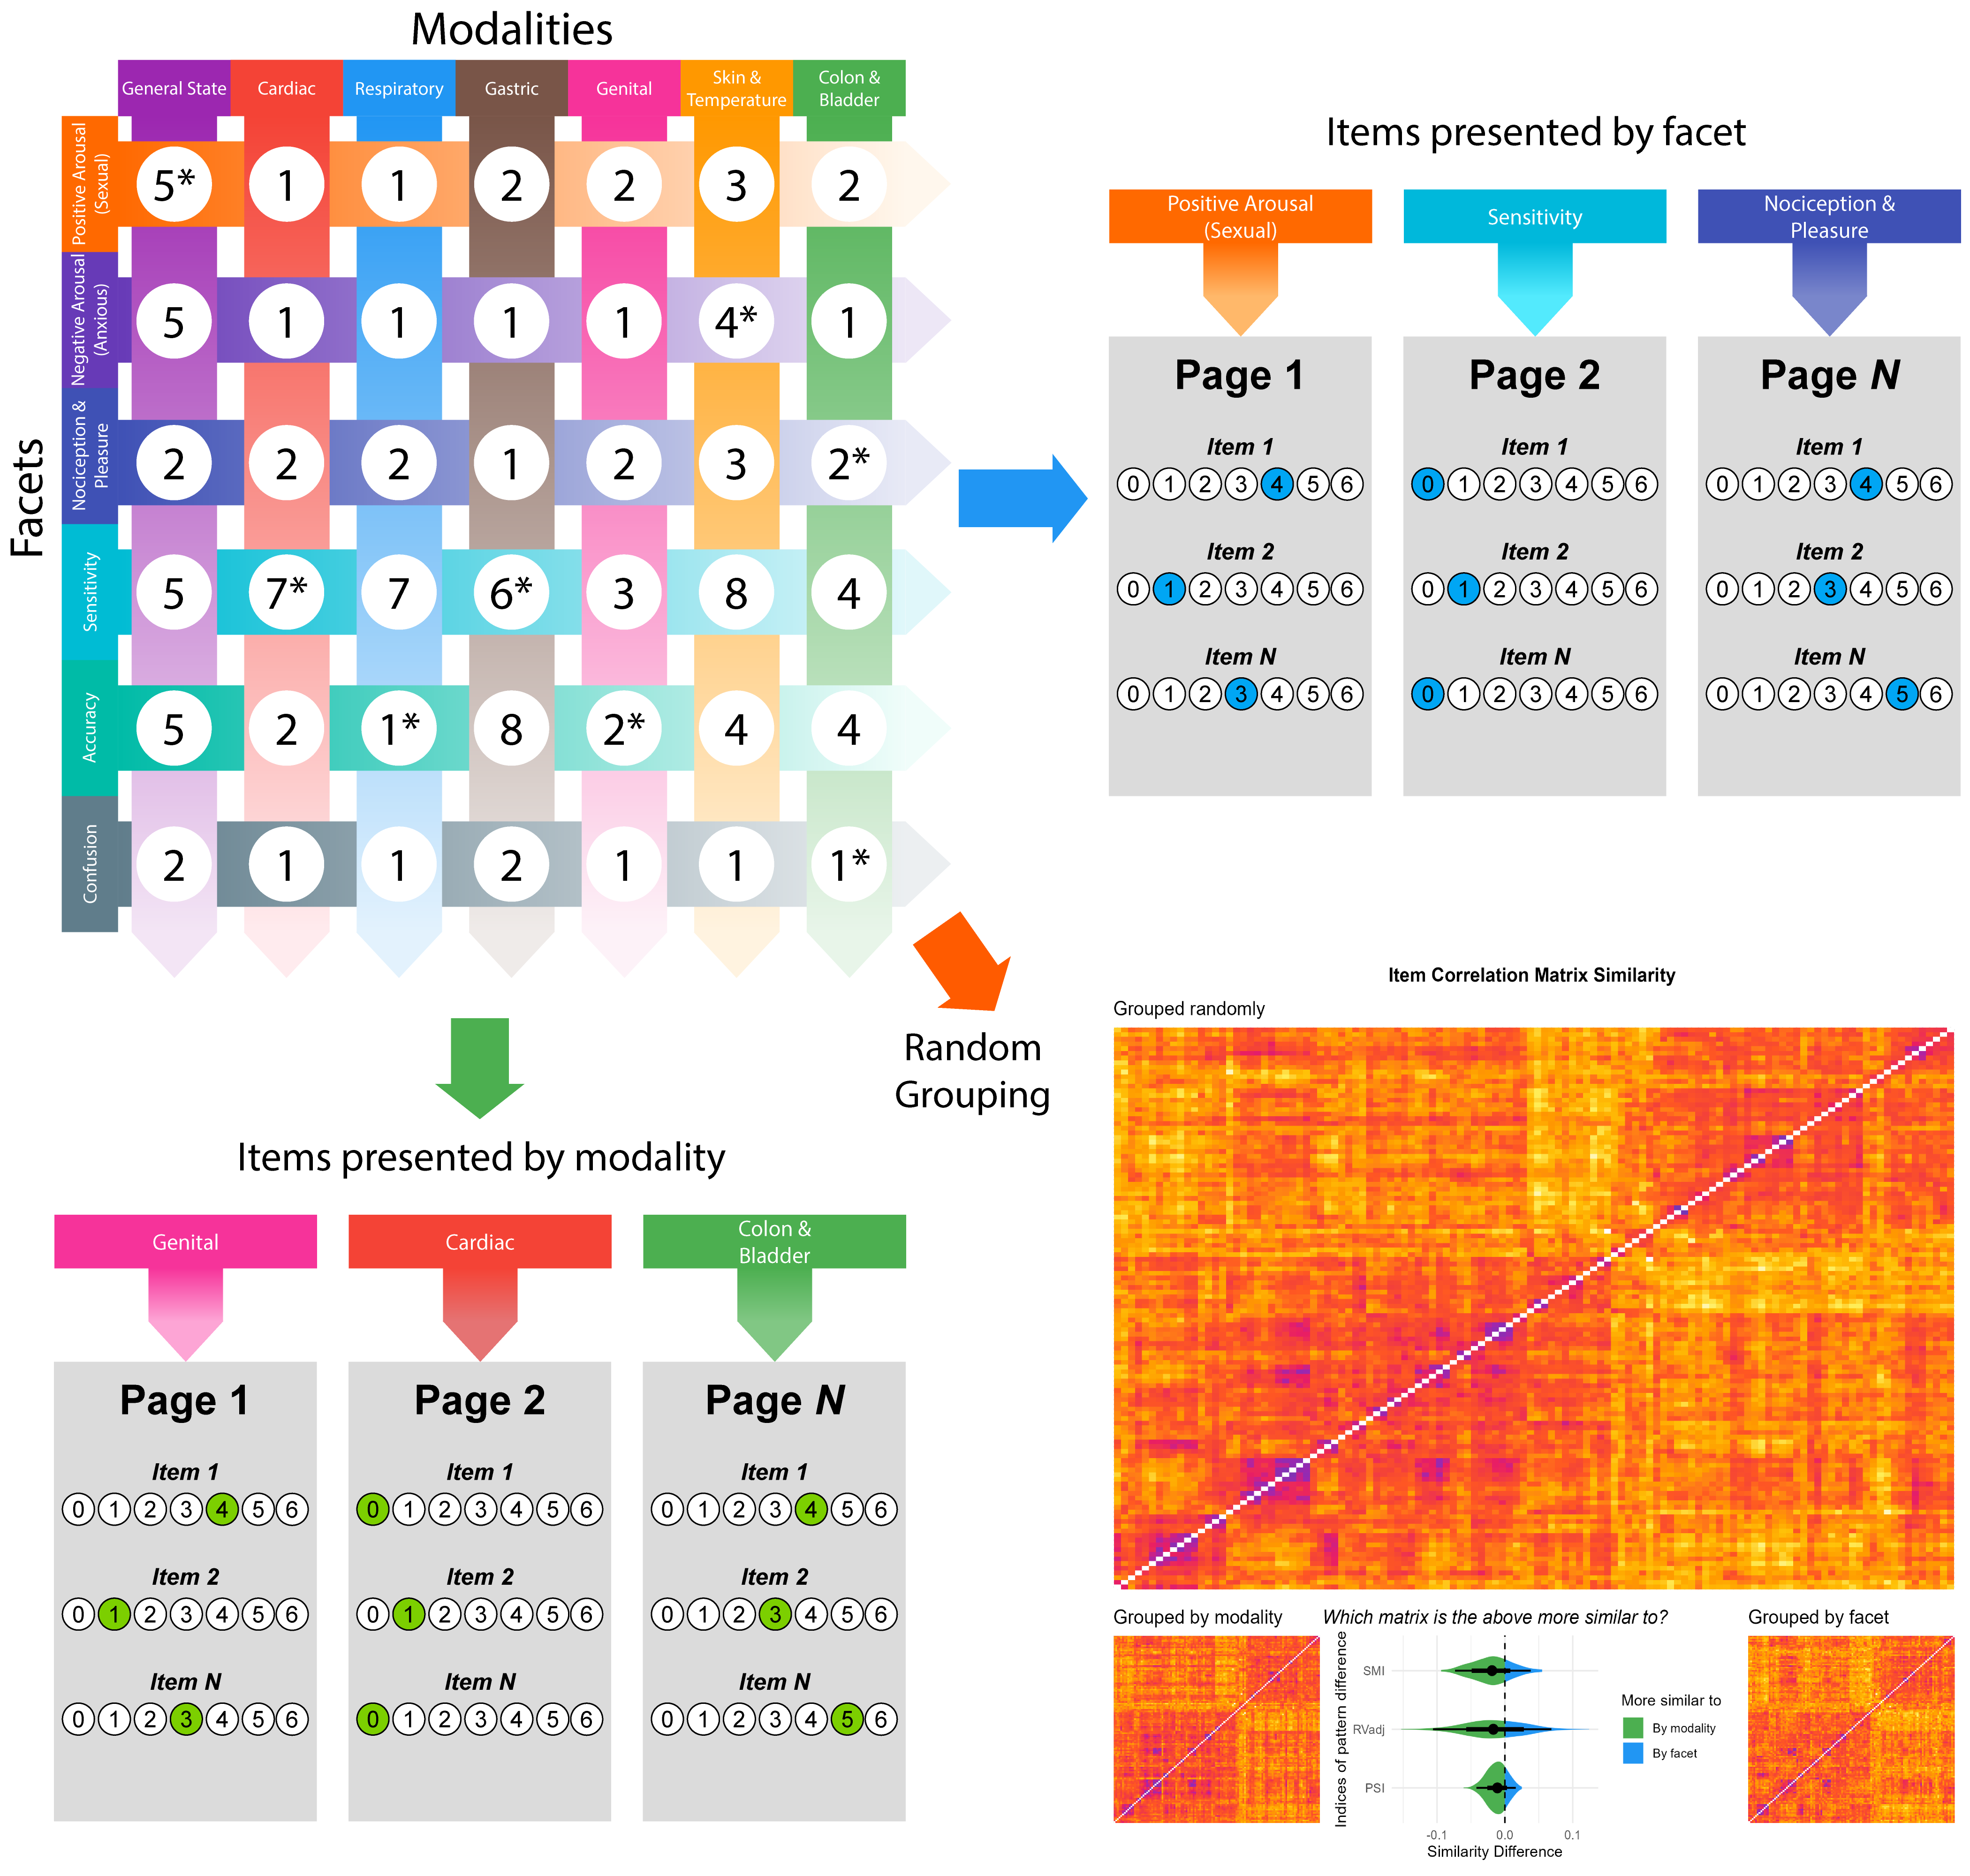
\includegraphics[width=1\linewidth,height=\textheight,keepaspectratio]{../study1/analysis/figures/figure1.png}
\end{center}

\end{figure*}

We identified 7 ``modalities'' (cardiac, respiratory, gastric, genital,
skin \& temperature (thermoregulation), bladder \& colon, and a
``general state'' category corresponding to a holistic and general
awareness of an interoceptive state or dimension). Through iterative
refinement (e.g., splitting or merging different categories together),
we settled on 6 ``facets'', which encompass both \emph{contexts} of
experience (negative and positive arousal, e.g., anxious and sexual
states), and potential distinct \emph{mechanisms} (nociception \&
pleasure, sensitivity, accuracy, and confusion).

Using this orthogonal 7x6 modality/facet grid as a conceptual
scaffolding, we generated 120 initial items, striving for a balanced
number of items with consistent phrasing within modalities and
facets\footnote{The initial item list is available at
  \href{https://realitybending.github.io/InteroceptionScale/study1/analysis/2_analysis.html}{realitybending.github.io/InteroceptionScale/study1/analysis/2\_analysis.html}}.
We additionally crafted 8 ``attention check'' items blending in (and
distributed across) each category.

\subsubsection{Procedure}\label{procedure}

To avoid presenting all the 120 items on a single long and discouraging
page, we split them into different pages. Participants were randomly
assigned to one of three conditions, driving how items were grouped on
the same page: 1) items grouped by modality (i.e., all cardiac items on
the first page, all colon \& bladder items on the second, etc.), 2)
items grouped by facet, or 3) items presented fully randomly (but with
their number balanced across 6 pages). The order of the item on any
given page and the order of the modalities/facets was randomized. Each
participant completed the full set of 120 items, with 8 attention check
items interspersed throughout. The online experiment was implemented
using JsPsych (\citeproc{ref-de2015jspsych}{De Leeuw, 2015}), and item
responses were recorded using 7-points Likert scales (0 = Disagree, 6 =
Agree).

\subsubsection{Data Analysis}\label{data-analysis}

In order to test whether the grouping condition had an effect on the
structure (i.e., how items relate to one-another), we compared the
correlation matrix obtained in the random condition to the ones obtained
in the modality and facet conditions, focusing on 3 indices of
correlation matrix similarity - the Procrustes Similarity Index (PSI,
\citeproc{ref-sibson1978studies}{Sibson, 1978}), the Adjusted RV (Rvadj,
\citeproc{ref-mayer2011exploratory}{Mayer et al., 2011}), and the
Similarity of Matrices Index (SMI,
\citeproc{ref-indahl2018similarity}{Indahl et al., 2018}). For each
index, we bootstrapped the difference between the similarity with the
facet and modality conditions to test whether the correlation matrix in
the random-grouping condition is significantly more similar to any of
the two other conditions.

Items deemed ``redundant'' (which can distort the item structure
estimation by introducing multicollinearity or local dependencies) were
identified (using the recommended threshold of 0.25) using Unique
Variable Analysis (UVA, \citeproc{ref-christensen2023unique}{Christensen
et al., 2023}), a novel and principled method derived from network
psychometrics.

The structure of the items was analyzed using the recently-developed
Exploratory Graph Analysis (EGA, \citeproc{ref-golino2017exploratory}{H.
F. Golino \& Epskamp, 2017}) framework, which allows to jointly estimate
the number of dimensions (i.e., clusters of items), the structure, as
well as its stability using bootstrapping
(\citeproc{ref-golino2020investigating}{H. Golino et al., 2020}). At a
fundamental level, EGA conceptualizes variables as nodes in a network,
with connections (edges) reflecting associations between them. Evidence
has underlined its suitability as an alternative to traditional factor
analysis, addressing some of its limitations such as the assumption of a
``latent'' source of variability, issues in estimation of the optimal
factor numbers, and poor performance in complex population structures,
while remaining comparable and interpretable
(\citeproc{ref-christensen2021equivalency}{Christensen \& Golino,
2021b}; \citeproc{ref-jimenez2023dimensionality}{Jiménez et al., 2023}).
In particular, nodes communities (i.e., clusters of items) can be in
practice interpreted as distinct ``dimensions'', similarly to
traditional latent factors - but without explicitly assuming their
existence (\citeproc{ref-christensen2021equivalency}{Christensen \&
Golino, 2021b}).

After removing redundant items using UVA, we iteratively fitted
hierarchical EGA models (which additionally estimate higher-order
``meta'' clusters) using ``glasso''
(\citeproc{ref-friedman2008sparse}{Friedman et al., 2008}) and the
``Leiden'' algorithm (\citeproc{ref-traag2019louvain}{Traag et al.,
2019}) for community detection, refining the item pool at each step. We
started by removing items with a low (\textless{} 80\%) cluster
stability (i.e., volatile items which jump between clusters across
bootstrapped samples), followed by odd items belonging to no clusters or
pairs of items (i.e., we keep items belonging to clusters of more than 2
items). Finally, for each lower-level cluster, we selected the 3 items
with the highest node centrality (i.e., the highest loading in the
cluster).

For both studies, data analysis was carried out using R (4.4.3,
\citeproc{ref-Rcoreteam}{R Core Team, 2025}), leveraging the
\emph{easystats} ecosystem (\citeproc{ref-ludecke2019insight}{Lüdecke et
al., 2019}, \citeproc{ref-ludecke2020extracting}{2020}) and the
\emph{EGAnet} package
(\citeproc{ref-christensen2021estimating}{Christensen \& Golino,
2021a}). The reproducible code and additional details are available at
https://github.com/RealityBending/InteroceptionScale.

\subsection{Results}\label{results}

The correlation matrix similarity analysis yielded no significant
differences between the similarity of the random-grouping condition with
the modality-grouping and facet-grouping conditions
(\(PSI_{\text{Random vs. Facet}} = 0.81\),
\(PSI_{\text{Random vs. Modality}} = 0.82\), \(p = .45\);
\(RVadj_{\text{Random vs. Facet}} = 0.77\),
\(RVadj_{\text{Random vs. Modality}} = 0.78\), \(p = .74\);
\(SMI_{\text{Random vs. Facet}} = 0.49\),
\(SMI_{\text{Random vs. Modality}} = 0.51\), \(p = .52\)), despite a
consistent bias in favour of the modality-grouping condition.

From the 120 initial items, 4 redundant items were flagged by UVA. We
then removed 40 items that showed low cluster stability, and 9 items
that were part of clusters with less than 3 items. Finally, We kept the
3 items with the highest loading in their lower-level structure
(removing 13 items in the process), resulting in 54 items in the final
item pool.

The final hierarchical EGA model (Generalized Total Entropy Fit Index =
-119.18) - in which all 54 items yielded a high cluster stability
(\textgreater{} 90\%) suggested 3 metaclusters and 15 lower-level
clusters (each containing 3 items): ``Interoceptive Deficits''
(containing 5 clusters: \emph{Urointestinal Inaccuracy} - UrIn;
\emph{Cardiorespiratory Confusion} - CaCo; \emph{Cardiorespiratory
Noticing} - CaNo; \emph{Olfactory Compensation} - Olfa; \emph{Satiety
Noticing} - Sati), ``Interoceptive Awareness'' (containing 7 clusters:
\emph{Sexual Arousal Awareness} - SexA; \emph{Sexual Arousal
Sensitivity} - SexS; \emph{Sexual Organs Sensitivity} - SexO;
\emph{Urointestinal Sensitivity} - UrSe; \emph{Relaxation Awareness} -
RelA; \emph{State Specificity} - StaS; \emph{Expulsion Accuracy} -
ExAc), and ``Interoceptive Sensitivity'' (containing 6 clusters:
\emph{Cardioception} - Card; \emph{Respiroception} - Resp;
\emph{Signalling} - Sign; \emph{Gastroception} - Gast; \emph{Dermal
Hypersensitivity} - Derm; \emph{Sexual Arousal Changes} - SexC).

To further reduce and balance the remaining items, we collectively
decided on removing the lower-level clusters \emph{Sexual Arousal
Awareness} (too general and overlapping with the other more specific
sex-related items), \emph{Signalling} (which items started with ``when
something important is happening in my life'', which meaning we deemed
too open to interpretation), and \emph{Sexual Arousal Changes} (low fit
with the other modality-focused clusters of its group). The final set
included 45 items.

\subsection{Discussion}\label{discussion}

The aim of Study 1 was to develop and refine a large, systematically
generated pool of interoceptive items into a psychometrically sound and
structurally coherent questionnaire. Starting with 120 items derived
from a modality-by-context grid, we employed a multi-step, data-driven
reduction process using cutting-edge structure analysis methods. This
procedure yielded a final, balanced set of 45 items, organised within a
stable hierarchical structure comprising three higher-order dimensions
(Interoceptive Deficits, Interoceptive Awareness, Interoceptive
Sensitivity) and 12 distinct lower-level facets.

The resulting hierarchical structure offers novel yet interpretable
insights into self-reported interoception, with flexible degrees of
granularity. Notably, we categorised several facets (typically related
to objective external behaviours, like coughing or sneezing) under the
label ``Awareness''. Although other questionnaires might refer to this
as ``Accuracy'', we preferred to preserve the notion that subjective
self-reports, by their very nature, cannot be a pure measure of
objective accuracy and are, at best, a proxy for subjective certainty or
awareness of interoceptive processes. Furthermore, our bottom-up
approach revealed intriguing facets, such as ``Olfactory Compensation''.
This finding provides evidence for a pseudo-interoceptive pathway,
whereby individuals with poorer access to internal signals may
compensate by relying on external cues (e.g., odours) to infer their
bodily state. The ``Sensitivity'' metacluster also grouped core
visceroceptive facets (e.g., ``Cardioception'', ``Gastroception'') with
``Dermal Hypersensitivity'', pointing to a potential common dimension of
heightened perceptual sensitivity to bodily sensations.

An additional innovation of Study 1 was examining the effect of item
presentation on the resulting psychometric structure by comparing
structures across different grouping conditions. Although there were no
significant effects of item presentation, a consistent (though
non-significant) trend suggested that grouping items by modality (rather
than by facet or randomly) could be more conducive to revealing the
underlying psychometric structure. This finding, while preliminary due
to the sample size per condition (\(N \pm 200\)), highlights a
potentially important and under-investigated aspect of questionnaire
design worthy of future research.

\section{Study 2: Validation}\label{study-2-validation}

Study 1 successfully leveraged a systematic item generation process and
modern analytical techniques to produce a 45-item interoception
questionnaire with a clear, stable, and theoretically rich hierarchical
structure. Study 2 then sought to formally validate the Mint scale by
examining its psychometric properties and its relationship with existing
measures in a large, independent sample. To this end, we sought to 1)
re-assess the structure of the shorter Mint version and 2) establish its
convergent validity by examining correlations with other established and
popular interoception questionnaires (namely the MAIA-2, BPQ, and IAS),
as well as other related measures (e.g., alexithymia). Finally, we
assessed the Mint's criterion validity by directly comparing the
predictive power of all interoception questionnaires across a broad
range of outcomes, including emotional, cognitive, and clinical
variables.

\subsection{Methods}\label{methods-1}

\subsubsection{Participants}\label{participants-1}

We recruited 921 English-speaking participants via SONA and
Prolific\textcopyright, from which 118 were excluded for failing at
least one attention check and 6 based on multivariate distance (using
the same procedure as for study 1). 60 participants were further
excluded due to missing data following a technical issue. The final
sample includes 737 participants (age = 36.8 \(\pm\) 14.7 {[}18, 87{]};
57.3\% women; Country of residence: 75.17\% United Kingdom, 24.83\%
other). This study was approved by the University of Sussex' Ethics
Committee (ER/EB672/2).

\subsubsection{Measures}\label{measures}

\begin{figure*}[!htbp]

{\caption{{Structure analysis of the final set of 33 Mint items.
Hierarchical Exploratory Graph Analysis (EGA) was applied to jointly
identify clusters of items, as well as higher-order metaclusters. The
reliability of each item can be quantified by the proportion of
structure replication across bootstrapped samples, with high values
indicative of high structural stability. The Mint scale displayed an
excellent structural consistency, with the exception of the \emph{Olfa}
cluster which belonging to the \emph{Deficit} metaclusters warrants
further research. Bottom plot shows the result of hierarchical
clustering, providing evidence for structure statbility across methods,
and allowing for more granular understanding of the relationships
between variables.}{\label{fig-two}}}}

\begin{center}
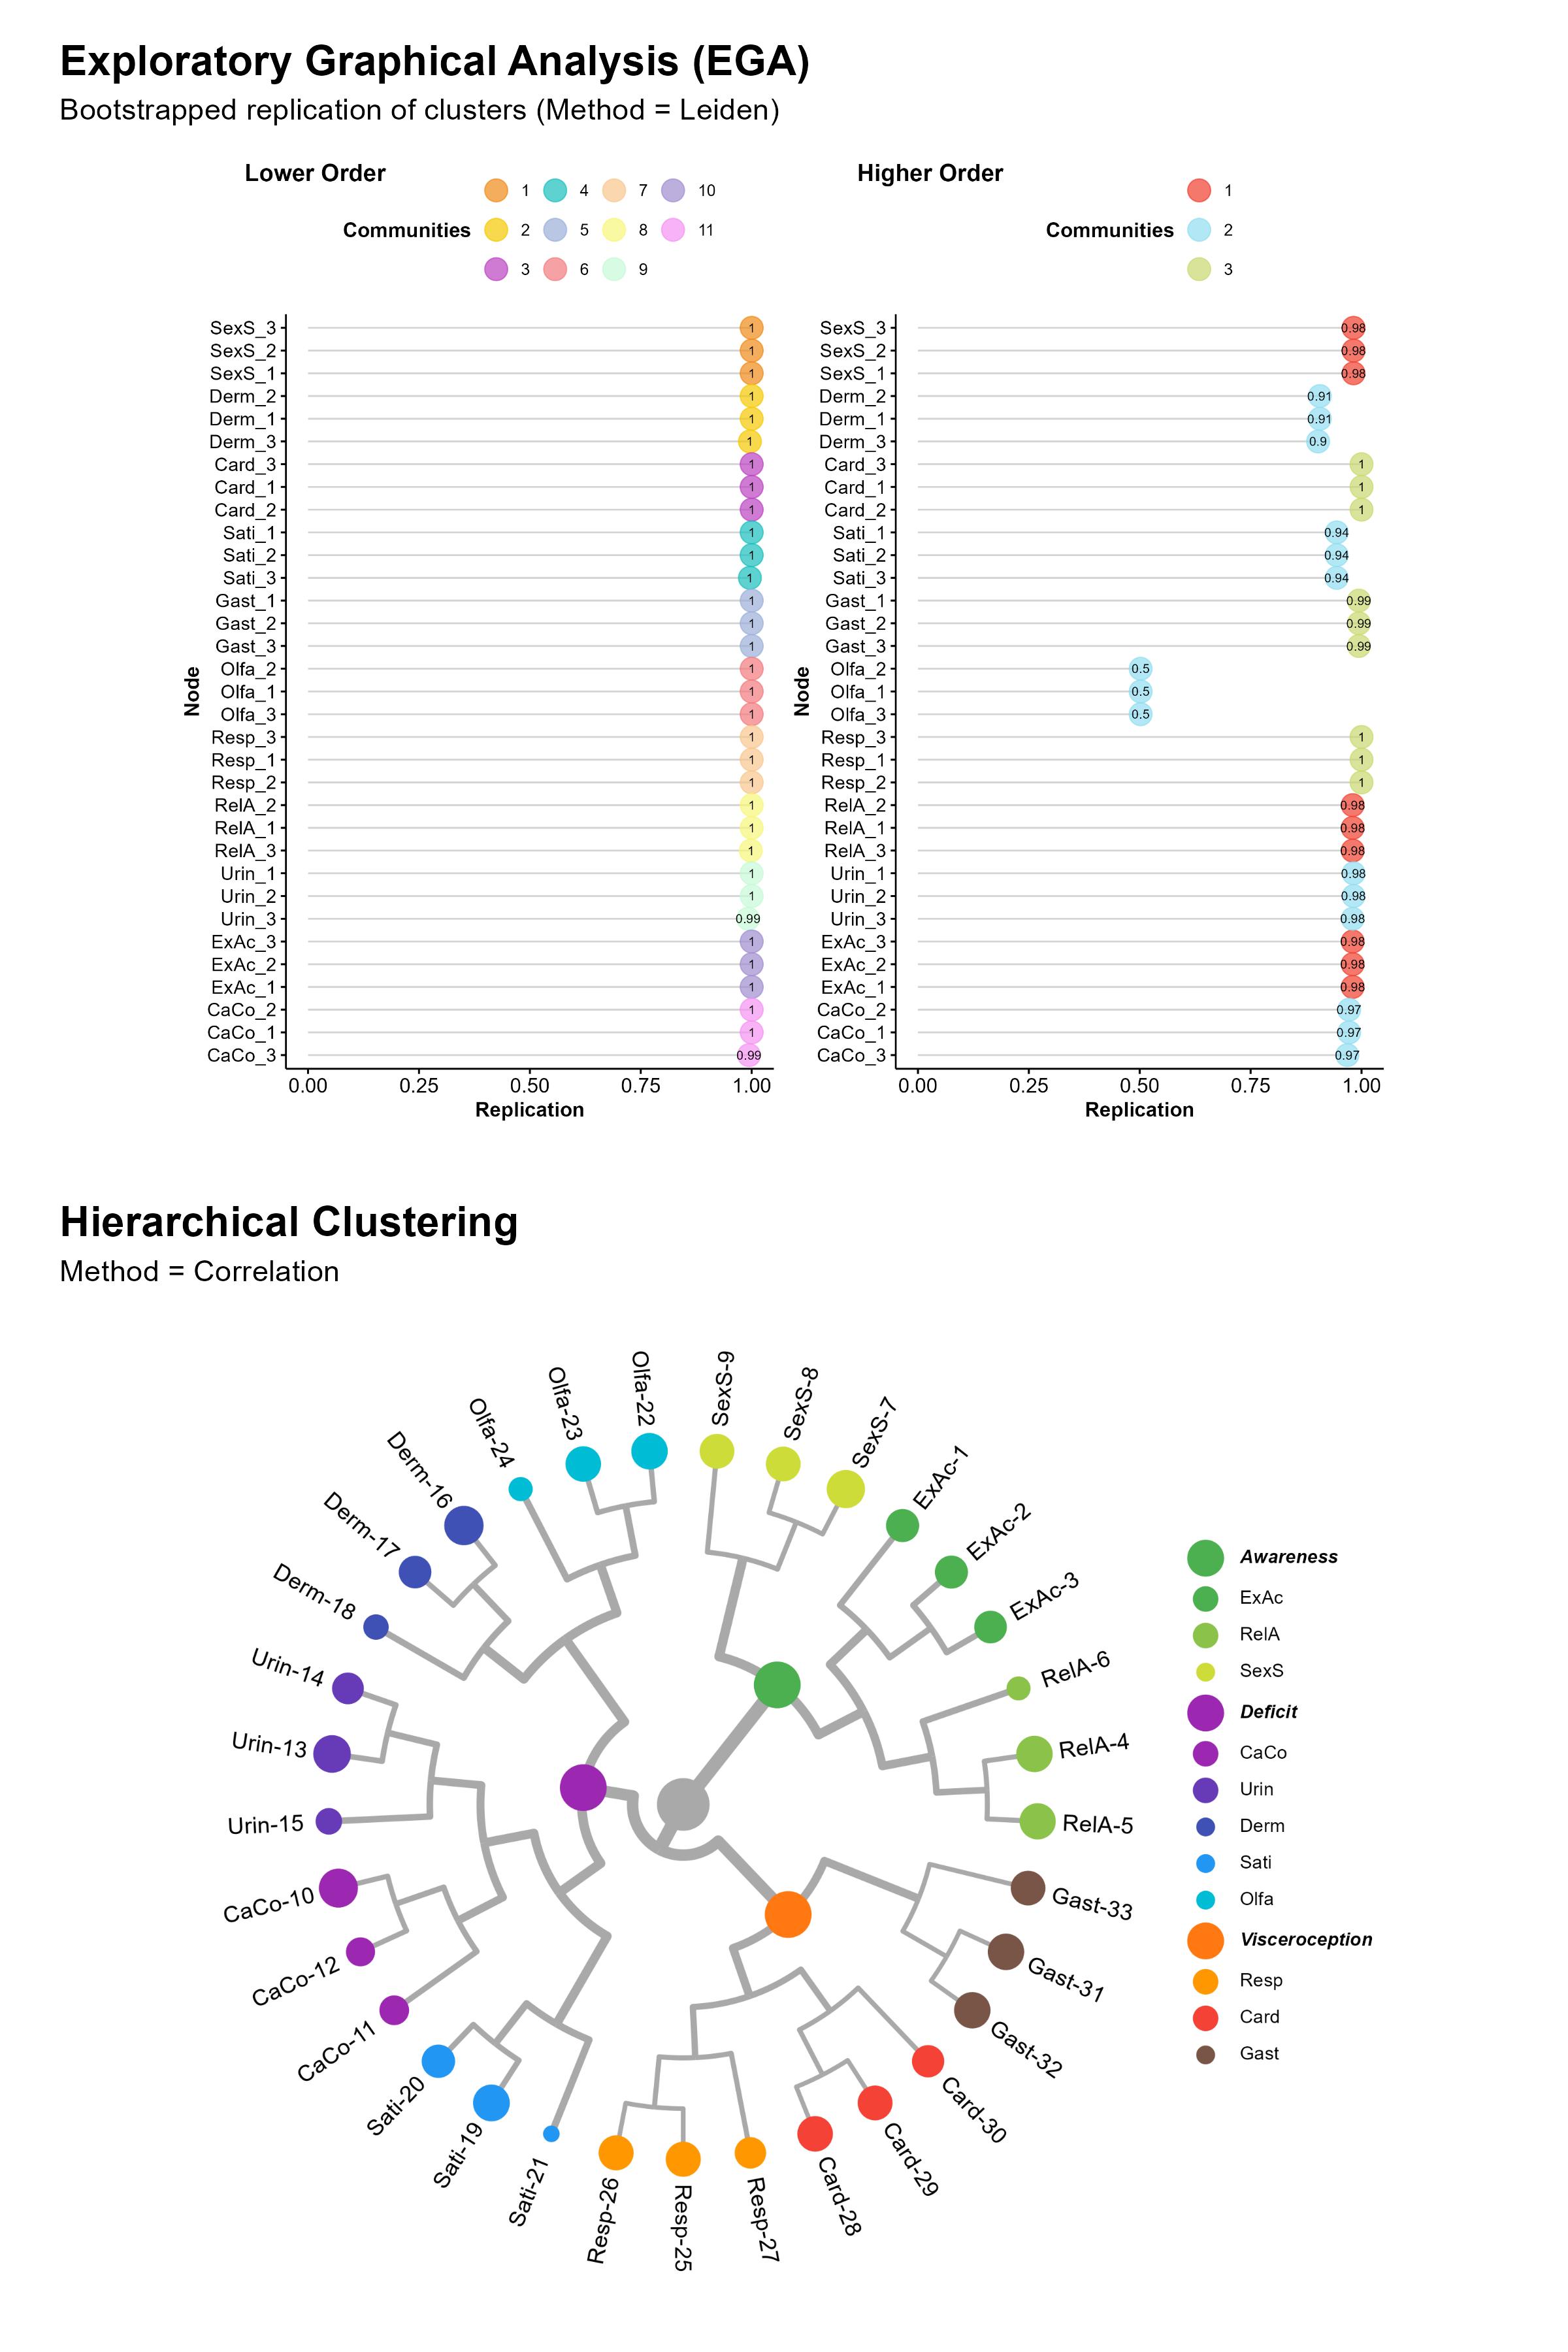
\includegraphics[width=0.8\linewidth,height=\textheight,keepaspectratio]{../study2/analysis/figures/fig1.png}
\end{center}

\end{figure*}

\paragraph{Interoception
Questionnaires.}\label{interoception-questionnaires}

The 45 items of the Multimodal Interoception Questionnaire (Mint) scale
were presented in a random order, with the same 7-point Likert scale as
in study 1 (0 = \emph{Disagree}, 6 = \emph{Agree}).

The Multidimensional Assessment of Interoceptive Awareness (MAIA-2,
\citeproc{ref-mehling2018multidimensional}{Mehling et al., 2018})
measures 8 dimensions with 37 items presented on a 7-point Likert scale
(0 = \emph{Never}, 6 = \emph{Always}). It includes bodily dimensions
such as Body Listening, Noticing, Emotional Awareness, dimensions
related to emotion regulation, such as Trust, Not-worrying, and
Self-Regulation, as well as dimensions related to attention, such as
Attention Regulation and Not-Distracting. The relationship of some of
these dimensions to interoception remains debated, particularly
Not-Distracting and Not-Worrying, which tend to show weak or
non-existent correlations with the other MAIA subscales
(\citeproc{ref-ferentzi2021examining}{Ferentzi et al., 2021}).

The Body Perception Questionnaire - Very Short Form (BPQ-VSF,
\citeproc{ref-cabrera2018assessing}{Cabrera et al., 2018}) measures a
general score of bodily awareness with 12 items presented on 5-point
Likert scale (0 = \emph{Never}, 5 = \emph{Always}).

The Interoceptive Accuracy Scale (IAS,
\citeproc{ref-murphy2020testing}{Murphy et al., 2020}) measures a
general score of interoceptive accuracy to physical sensations with 21
items presented on a 5-point Likert scale (1 = \emph{Disagree Strongly},
5 = \emph{Strongly Agree}).

\paragraph{Emotions and Cognition.}\label{emotions-and-cognition}

The Toronto Alexithymia Scale TAS (TAS-20,
\citeproc{ref-leising2009toronto}{Leising et al., 2009}) measures 3
Alexithymia dimensions with 20 items 5-point Likert scale (1 =
\emph{Strongly Disagree}, 5 = \emph{Strongly Agree}: Difficulty
Identifying Feelings (DIF), Difficulty Describing Feelings (DDF), and
Externally Oriented Thinking (EOR).

The Emotion Reactivity Scale - Brief Version (B-ERS,
\citeproc{ref-veilleux2024development}{Veilleux et al., 2024}) measures
3 dimensions with 6 items on a 5-point Likert scale (0 = \emph{Not like
me at all}, 4 = \emph{Extremely like me}): Arousal (\emph{``My moods are
very strong and powerful''}), Sensitivity (\emph{``I tend to get very
emotional very easily''}), and Persistence (\emph{``When I am
angry/upset, it takes me much longer than most people to calm down''}).

The Cognitive Emotion Regulation Questionnaire (CERQ-short,
\citeproc{ref-garnefski2006cognitive}{Garnefski \& Kraaij, 2006})
measures 9 adaptive and maladaptive emotion regulation strategies with
18 items (1 = \emph{Almost Never}, 5 = \emph{Almost Always}). The
strategies include Self-blame, Other-blame, Rumination, Catastrophizing,
Putting into Perspective, Positive Refocusing, Positive Reappraisal,
Acceptance, and Planning.

The Černis Felt Sense of Anomaly scale - short form (CEFSA-14,
\citeproc{ref-vcernis2024measuring}{Černis et al., 2024}) measures 7
dissociative experiences with 14 items on a 5-point Likert scale (0 =
\emph{Never}, 4 = \emph{Always}). This scale is designed to measure
dissociative experiences in adolescence and adulthood, specifically
focusing on the felt sense of anomaly-type dissociation. It includes
Anomalous Experience of the Self, Anomalous Experience of the Body,
Anomalous Experiences of Emotion, Altered Sense of Familiarity, Altered
Sense of Connection, Altered Sense of Agency, and Altered Sense of
Reality.

The Primal World Beliefs Inventory (PI-18,
\citeproc{ref-clifton2021brief}{Clifton \& Yaden, 2021}) measures
higher-order beliefs about the basic character of the world: Good, Safe,
Enticing, and Alive. The 18 items are presented on a 6-point Likert
scale (0 = \emph{Strongly Disagree}, 5 = \emph{Strongly Agree}).

\paragraph{Health and Wellbeing.}\label{health-and-wellbeing}

The Single Item Life Satisfaction scale (SILS,
\citeproc{ref-jovanovic2020longer}{Jovanović \& Lazić, 2020}) was
followed by the PHQ-4 (\citeproc{ref-kroenke2009ultra}{Kroenke et al.,
2009}) assessing depression and anxiety symptoms with 4 items. We used
the refined version of the PHQ-4
(\citeproc{ref-makowski2025measuring}{Makowski et al., 2025}), which
adds an additional response option (``Once or twice''), increasing
sensitivity to subclinical fluctuations.

Participants were asked to self-report any current, medically diagnosed
psychiatric disorders using a checklist based on DSM-5 categories. If
one or more conditions were endorsed, participants were asked to
indicate any current treatments, including pharmacological (e.g.,
antidepressants, anxiolytics, antipsychotics, mood stabilizers),
psychological (e.g., psychotherapy, mindfulness), or lifestyle
interventions. Binary variables (0 = absent, 1 = present) were created
to identify participants reporting mood disorders (Major Depressive
Disorder, Bipolar Disorder; with a stricter subgroup of participants
undergoing a pharma- or psychological treatment), anxiety-centred
disorders (Generalised Anxiety Disorder, Panic Disorder, Social Anxiety
Disorder, Specific Phobias), eating disorders, addiction-related
disorders, borderline personality disorder, autism spectrum disorder
(ASD), and ADHD.

Participants were asked to select somatic symptoms or conditions they
experienced from a list of 36 options. To facilitate mechanistic
interpretation and reduce redundancy, answers were grouped into four
non-overlapping clusters based on shared physiological pathways and
known etiological mechanisms. The \emph{Afferent Sensitivity} cluster
included conditions associated with heightened interoceptive awareness
and neurogenic excitability, such as migraine, neuropathy, dizziness,
nausea, muscle tension, epilepsy, and frequent urination. The
\emph{Central Sensitization} cluster comprised syndromes characterized
by chronic pain and fatigue, likely reflecting central amplification of
sensory signals and HPA-axis dysregulation, such as fibromyalgia,
chronic fatigue syndrome, chronic pain, back pain, pelvic pain,
irritable bowel syndrome (IBS). The \emph{Autonomic Dysfunction} cluster
captured disorders linked to dysregulation of the autonomic and
cardiopulmonary systems, including joint hypermobility, cardiac
arrhythmia, chest pain, shortness of breath, hypo-/hypertension, sleep
apnea, chronic obstructive pulmonary disease (COPD), and chronic
bronchitis. Finally, the \emph{Immune-Inflammatory} cluster encompassed
conditions associated with immune dysregulation, barrier dysfunction,
and gut-brain axis disturbance, such as eczema, psoriasis, skin rashes,
asthma, celiac disease, gluten and lactose sensitivity, inflammatory
bowel diseases (Crohn's disease and ulcerative colitis),
gastroesophageal reflux disease (GERD), multiple sclerosis, and
Sjögren's syndrome. We scored each cluster as a binary variable based on
whether the participant selected at least one symptom from that cluster.

\paragraph{Lifestyle.}\label{lifestyle}

Participants reported about owning any wearable devices to monitor
health indices such as heart rate, number of steps, calories burned,
sleep quality, and weight. For each selected device, a follow-up
question inquired about the frequency of usage and subjective importance
of that measure.

Participants were asked to rate how physically active they consider
themselves and how many hours of active workout they engage in per week.
Participant's BMI was computed using height and weight.

\subsubsection{Procedure}\label{procedure-1}

In order to avoid the repetition of similar types of questions and and
balance longer and shorter questionnaires, we partitioned the measures
into three groups (and randomized the order within them): 1)
interoception questionnaires (MAIA, IAS, BPQ), 2) emotions (TAS, CERQ,
ERS, PI-18), and 3) health (somatic symptoms, mental health, LS + PHQ-4,
CEFSA). After completing demographic questions, participants always
started with the Mint scale, and each following interoception
questionnaire was interspersed with two questionnaires from the emotions
and pathology groups. 7 attention checks were embedded throughout (one
within each major questionnaire). In order to make the experiment more
enjoyable, the experiment ended with a radar chart summarizing the
participants' responses to the Mint scale\footnote{The experiment can be
  tested by following the link on
  https://github.com/RealityBending/InteroceptionScale}.

\begin{figure*}[!htbp]

{\caption{{Item loadings. The table shows each item of the Mint with its
cluster centrality, which is the EGA equivalent (in terms of
interpretation) of factor loadings. It also shows how each lower-level
cluster is related to higher-order metaclusters. The lower-level
clusters are Expulsion Accuracy (ExAc), Relaxation Awareness (RelA),
Sexual Arousal Sensitivity (SexS), Cardiorespiratory Confusion (CaCo),
Urointestinal Inaccuracy (UrIn), Dermal Hypersensitivity (Derm), Satiety
Noticing (Sati), Olfactory Compensation (Olfa), Respiroception (Resp),
Cardioception (Card), Gastroception (Gast).}{\label{fig-three}}}}

\begin{center}
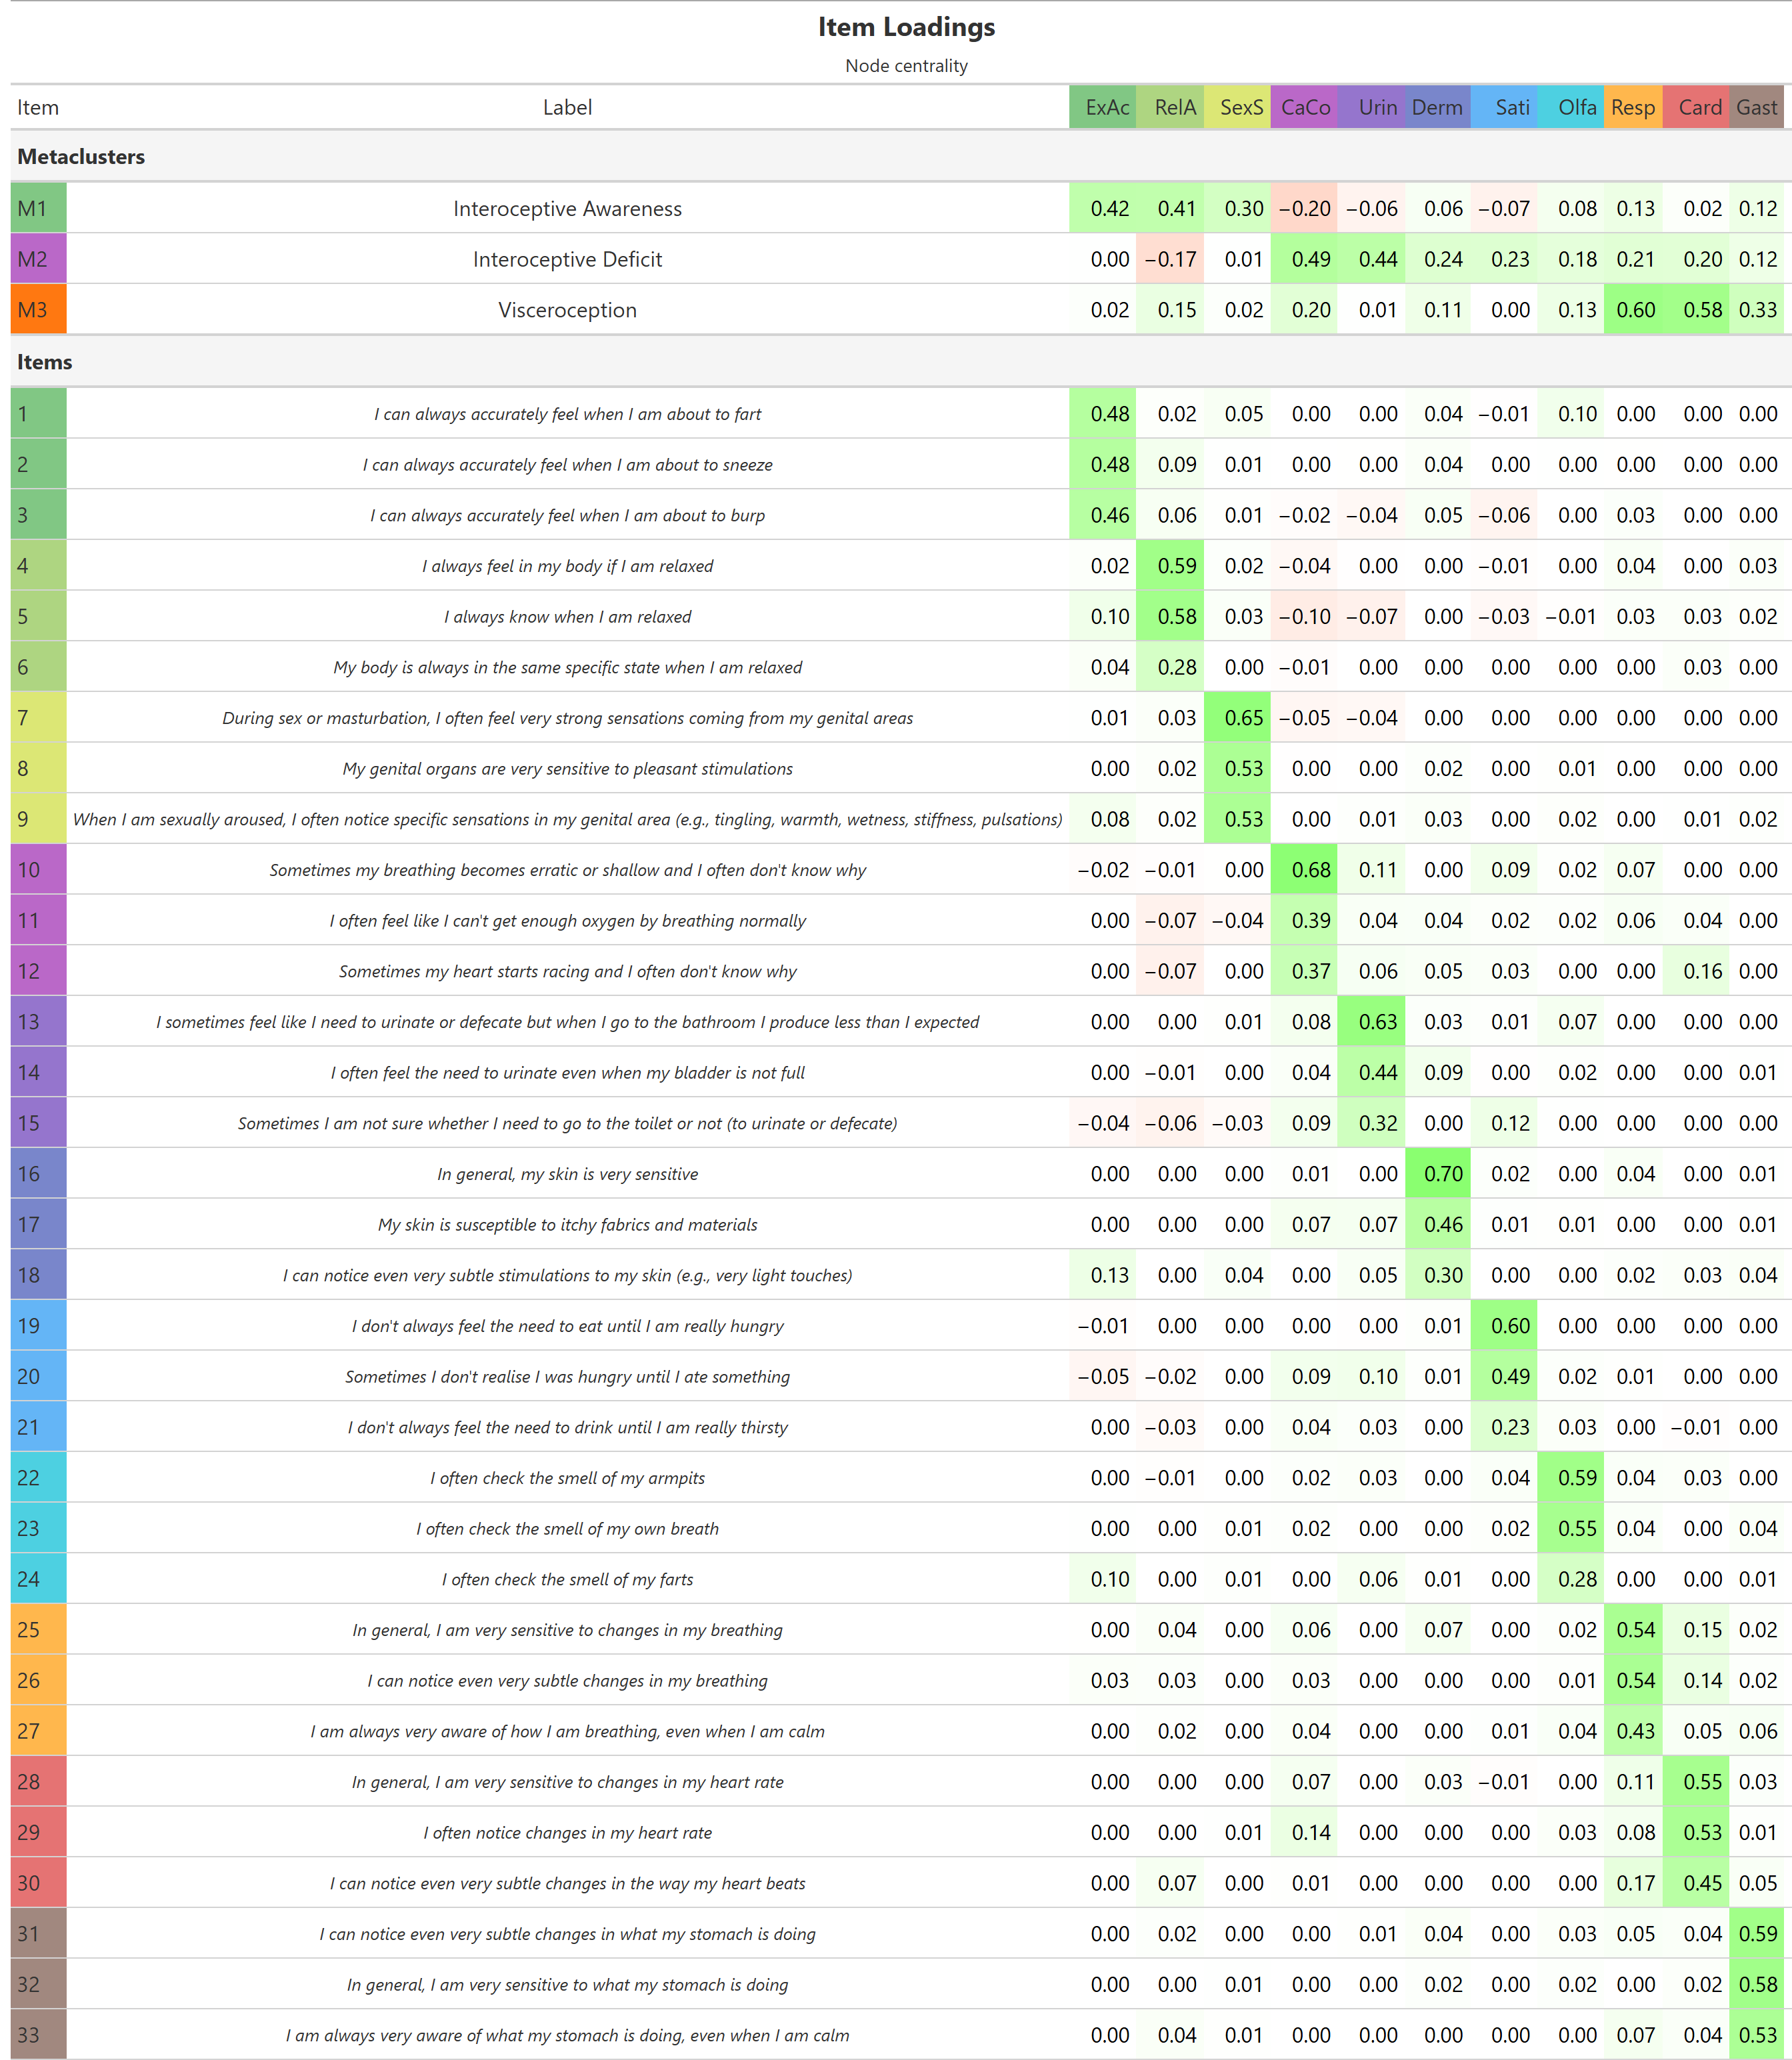
\includegraphics[width=1\linewidth,height=\textheight,keepaspectratio]{../study2/analysis/figures/table1.png}
\end{center}

\end{figure*}

\subsubsection{Data Analysis}\label{data-analysis-1}

We started by confirming and further refining the structure of the Mint
scale (see Figure~\ref{fig-two}) using the same EGA model as in Study 1.
We then computed the lower-level dimensions and the higher-level
metaclusters' scores by averaging their corresponding items. The
convergent validity of the final set of items was assessed by computing
the correlations between the Mint scale and the other interoception
questionnaires (MAIA, BPQ, IAS).

Next, we tested the predictive power of the Mint scale relative to other
interoception questionnaires. We assessed the importance of each
interoceptive dimension (from all the scales) as a unique predictor by
fitting regression models (linear for continuous measures - e.g.,
depression score - and logistic for binary variables - e.g., presence
\emph{vs.} absence of mood disorders) to predict different outcomes, and
compare the best between the 4 interoception scales based on the total
explained variance (R2 or pseudo-R2 for logistic models,
\citeproc{ref-ludecke2021performance}{Lüdecke et al., 2021}). We then
evaluated the predictive performance of each scale as a whole by
comparing regression models with all the dimensions entered as
predictors (note that the IAS and BPQ only have one total score
variable). We assessed the models based on their R2, as well as on the
Bayesian Information Criterion (BIC), which penalizes for predictor
number, thus offering a balance between model parsimony and predictive
power. For the logistic models, we quantified the discriminative power
by computing the Area Under the Curve (AUC) of the Receiver Operating
Characteristic (ROC) curve, which assesses the model's discriminative
power (the combination of sensitivity and specificity).

In order to evaluate the potential for a short version of our scale, we
compared 4 variants of the Mint: the (full) \emph{Mint} (including all
lower-level dimensions), the \emph{metaMint} (only including the
metaclusters), the \emph{miniMint} (including the metaclusters computed
from a reduced number of items), and the \emph{microMint} (including
only the most representative dimension of each metacluster). Moreover,
we also included an alternative ``interoception-focused'' version of the
MAIA (\emph{iMAIA}) that only contains the 3 most interoceptive
dimensions (Body Listening, Noticing, and Emotional
Awareness)\footnote{See correlation results to further justify this
  selection.}.

\subsection{Results}\label{results-1}

The application of EGA to the initial set of 42 items reproduced the
expected 14 lower-level clusters of triplets and 3 higher-order
metaclusters, with the exception of the \emph{UrSe} (Urointestinal
Sensitivity), for which one item moved to the \emph{Olfa} (Olfactory
Compensation) cluster. In order to further balance and reduce the items,
we removed the \emph{UrSe} cluster, as well as \emph{StaS} (State
Specificity), which in comparison to the other items stood out as
containing vague and overlapping items ; \emph{SexO} (Sexual Organs
Sensitivity), which overlapped with the \emph{SexS} (Sexual Arousal
Sensitivity) cluster; and \emph{CaNo} (Cardiorespiratory Noticing),
which overlapped with the \emph{CaCo} (Cardiorespiratory Confusion)
cluster.

The final set of 33 items yielded a good fit (Generalized Total Entropy
Fit Index = -77.23), with all items showing high cluster stability
(\textgreater{} 90\%), with the exception of \emph{Olfa}. The final
structure included 11 lower-level clusters, grouped into 3 higher-order
metaclusters: ``Interoceptive Deficit'' (containing \emph{CaCo},
\emph{UrIn}, \emph{Derm}, \emph{Sati}, \emph{Olfa}), ``Interoceptive
Awareness'' (containing \emph{ExAc}, \emph{RelA}, \emph{SexS}), and
``Visceroception'' (containing \emph{Card}, \emph{Resp}, \emph{Gast}).
Item centrality (intepretable as loadings in traditional factor analysis
frameworks) are shown in Figure~\ref{fig-three}. Additionally, we
applied hierarchical clustering analysis which replicated this structure
(see Figure~\ref{fig-two}), suggesting consistency across methods.

\begin{figure*}[!htbp]

{\caption{{Correlation Matrices between the Mint dimensions
(upper-left), and between the Mint and other interoception
questionnaires (MAIA, BPQ and IAS; upper-right). The bottom matrix shows
the relationships between interoception and other measures included in
the study, such as alexithymia (TAS-20), depression and anxiety (PHQ-4),
emotion reactivity (ERS), abnormal and dissociative experiences (CEFSA),
and Primal World Beliefs. Stars indicate dimensions that have been
score-reversed for better in-context interpretation. Correlation
coefficients are shown only for significant correlations (p \textless{}
.001).}{\label{fig-four}}}}

\begin{center}
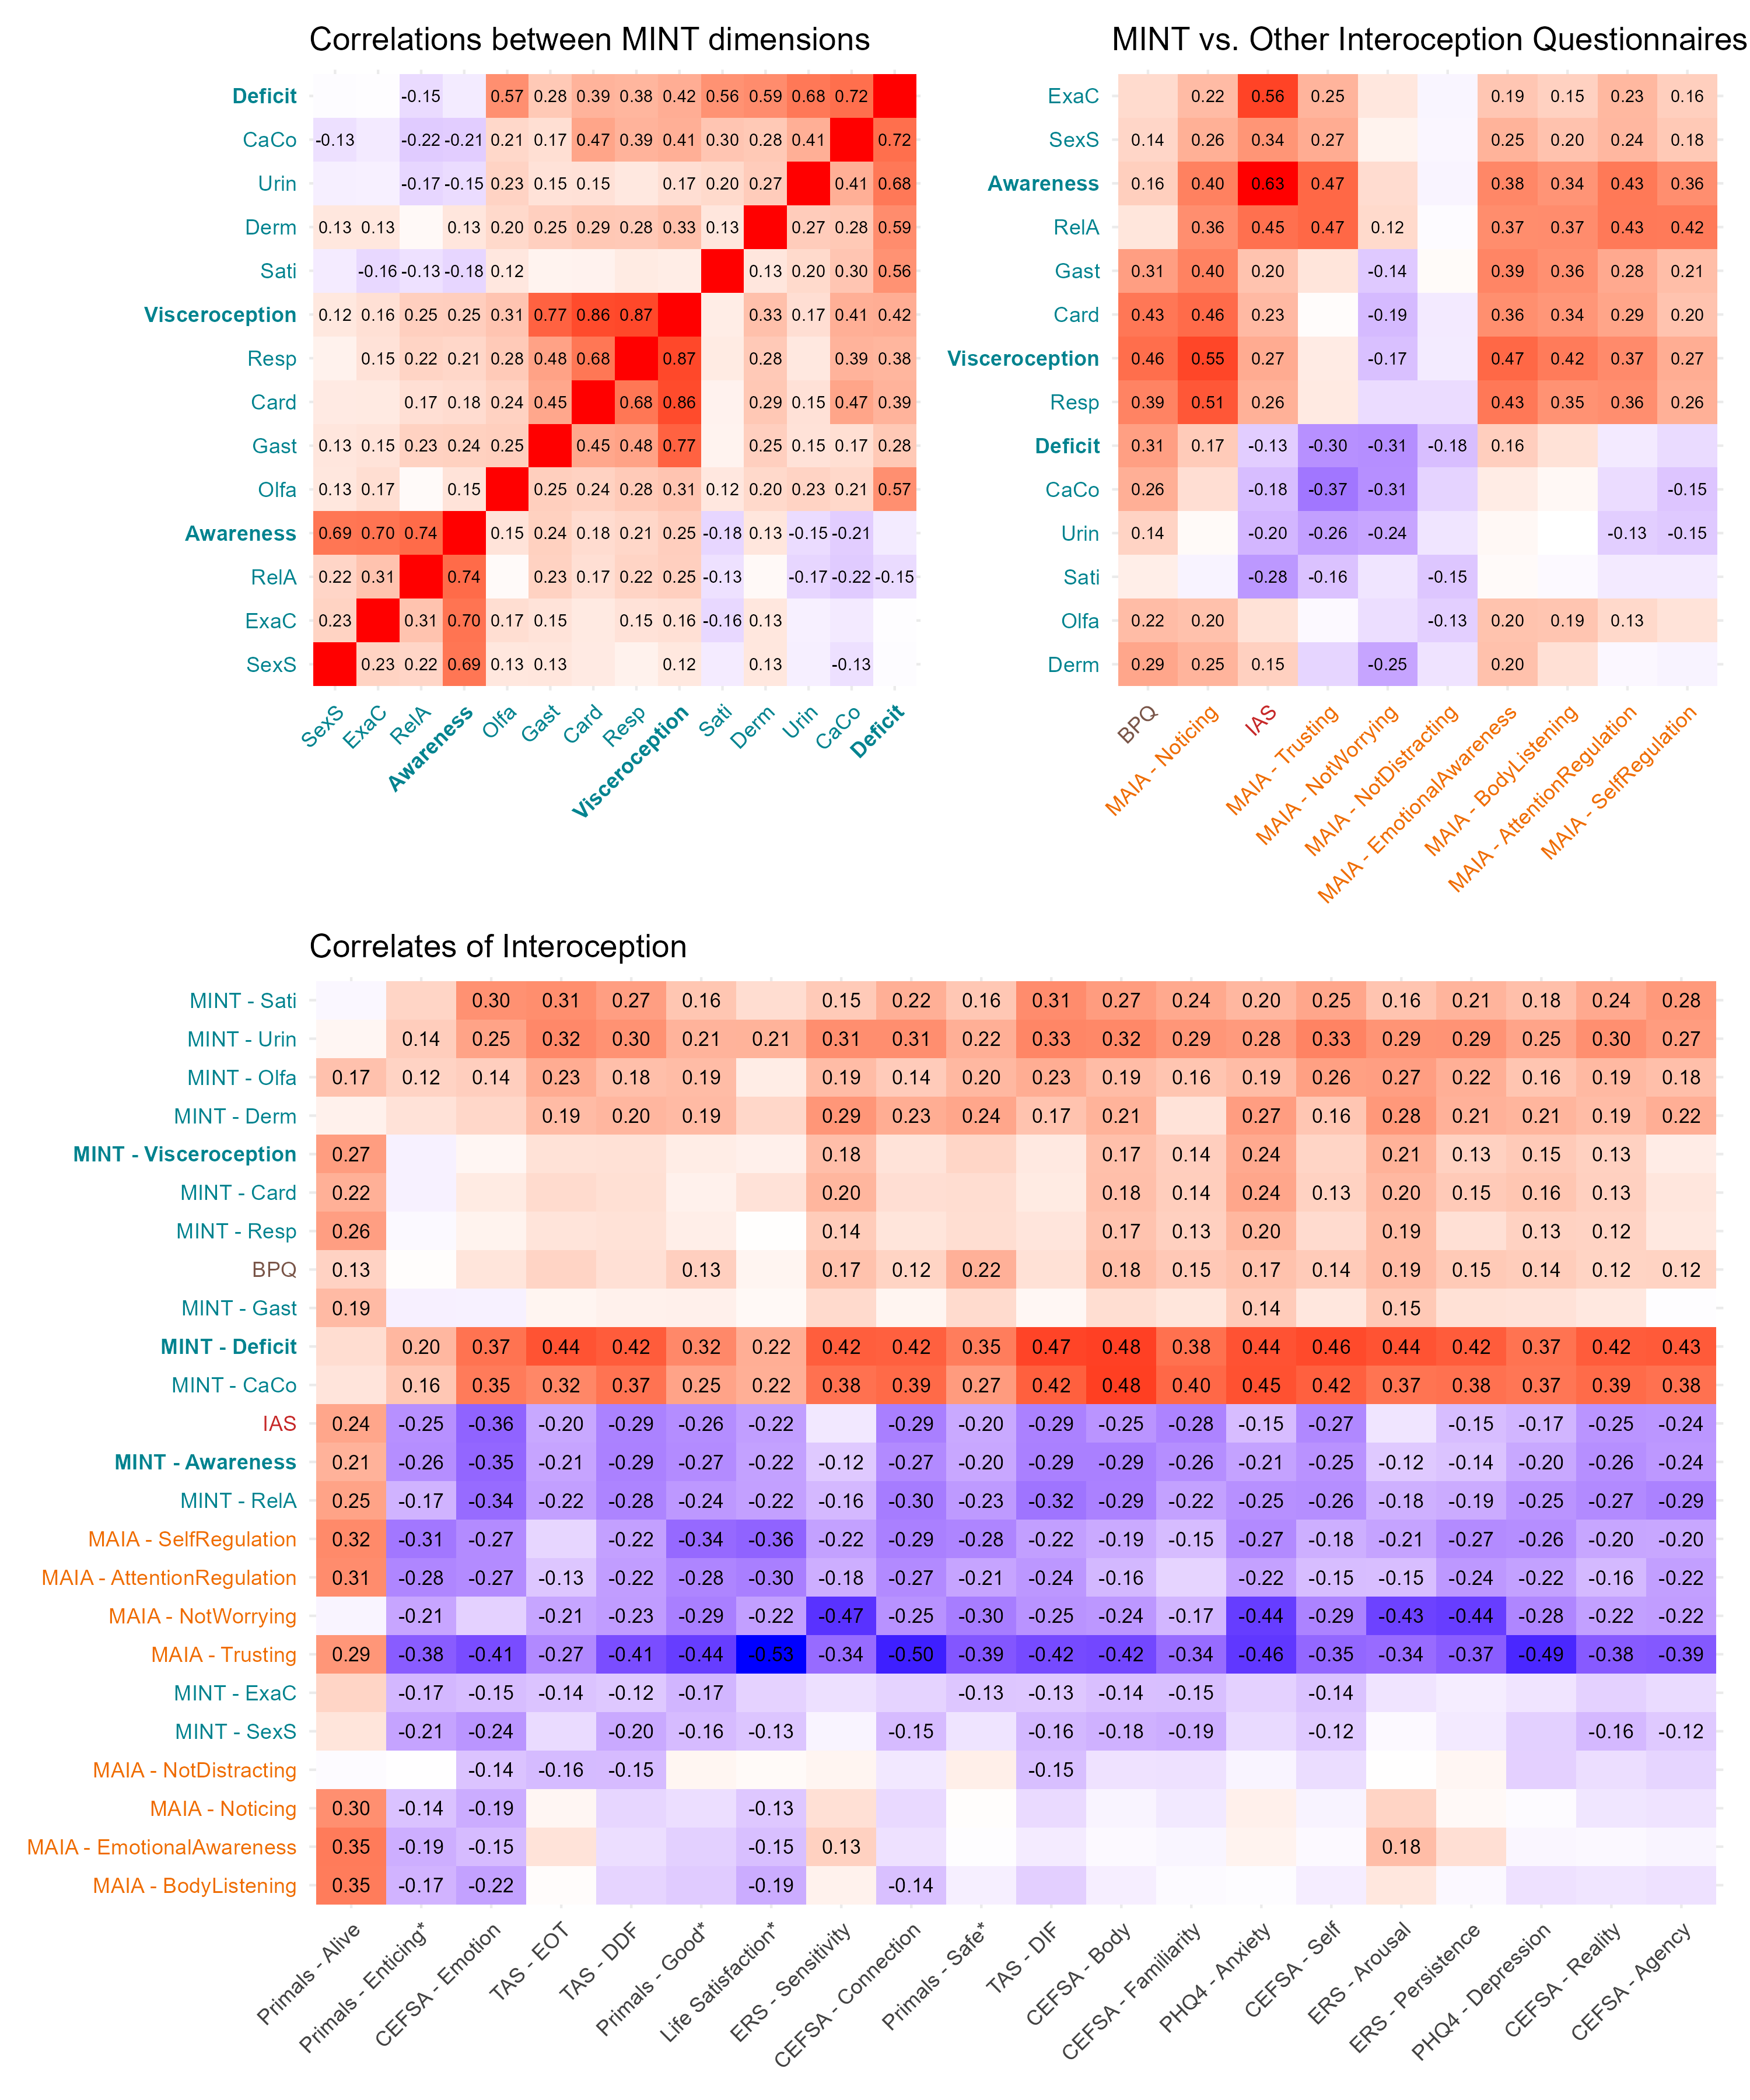
\includegraphics[width=1\linewidth,height=\textheight,keepaspectratio]{../study2/analysis/figures/fig2.png}
\end{center}

\end{figure*}

The correlation matrix of the Mint dimensions revealed an interesting
and rich tapestry of relationships (see Figure~\ref{fig-four}), with
contrasting patterns of associations with dimensions from the same
group. For instance, \emph{Derm} and \emph{Olfa}, despite being
positively correlated with the other dimensions from the \emph{Deficit}
cluster, were not negatively correlated to \emph{Awareness} and its
dimensions. Similarly, \emph{Sati}, unlike the other \emph{Deficit}
dimensions, was not positively correlated to \emph{Visceroception}. This
complex structure suggests that the dimensions indeed capture distinct
aspects of interoception, and that the metaclusters, rather than being
simple aggregates of rather-redundant elements, might actually capture
unique combinations (greater than the sum of their parts). It also
provides evidence against a simplistic adaptive \emph{vs.} maladaptive
dichotomy, as \emph{Deficit} was not negatively but positively
correlated with \emph{Visceroception}. Interestingly, while
\emph{Awareness} was also positively correlated with
\emph{Visceroception}, it yielded an insignificant negative correlation
with \emph{Deficit} (this finding was also aligned with the hierarchical
clustering results, showing a greater proximity between \emph{Deficit}
and \emph{Visceroception} than with \emph{Awareness}), underlining again
the complex web of relationships captured by the Mint.

The correlation matrix between the Mint and the other interoception
scales revealed high levels of overlap, as well as some unique
contributions (see Figure~\ref{fig-four}). The BPQ was positively
correlated with most Mint dimensions (the highest with
\emph{Visceroception}, \(r = .46\)). The IAS was positively correlated
with \emph{Visceroception} and \emph{Awareness} dimensions (the highest
with \emph{Awareness}, \(r = .63\)), but negatively with most
\emph{Deficit} dimensions (with the exception of \emph{Olfa} and
\emph{Derm}). In turn, the \emph{Visceroception} metacluster most
strongly correlated with MAIA's Noticing (\(r = .55\)). Interestingly,
MAIA's TTrusting correlated selectively with \emph{Awareness}, and
negatively with \emph{Deficit} dimensions, but not with
\emph{Visceroceptive} dimensions (underlining its high-level
metacognitive nature). MAIA's Emotional Awareness and Body Listening
displayed a similar pattern to Noticing, and Attention Regulation and
Self Regulation positively correlated with \emph{Awareness} and
\emph{Visceroception} dimensions, but negatively with some
\emph{Deficit} dimensions (\emph{CaCo} and \emph{UrIn}). Not-distracting
only yielded mild negative associations with \emph{Sati} and
\emph{Olfa}. Overall, the Mint dimensions were able to capture most of
the (relevant) variance and intricacies present in the other
interoception scales.

Exploratory correlations with the emotion regulation (CERQ) dimensions
revealed stronger associations with most of the MAIA dimensions
(supporting its proximity with emotion regulation). Interestingly,
Rumination (and Self-Blame) stood out as selectively related to the
Mint's \emph{Visceroception} and \emph{Deficit} dimensions (note that
Rumination was also related to the MAIA's interoceptive dimensions,
namely Noticing, Emotional Awareness and Body Listening). The only
primal world belief that correlated particularly with the Mint's
\emph{Visceroception} and the MAIA's interoceptive dimension was the
belief that the world was alive (i.e., the belief that the universe is
conscious, purposeful, and in active relationship with oneself,
\citeproc{ref-clifton2021brief}{Clifton \& Yaden, 2021}).

\begin{figure*}[!htbp]

{\caption{{Summary table of the comparison between interoception
questionnaires (Mint, MAIA, BPQ and IAS). For various outcomes included
the study, we tested the Mint and Non-Mint dimension that had the
strongest link (as a unique predictor). Values in parenthesis represents
correlation coefficient for continuous variables and log-odds ratios for
binary variables (the occurrence of mental and somatic health
conditions). We also compared the predictive performance of regression
models including multiple predictors, and present their ranking based on
raw predictive power (R2) and BIC, which favours more parsimonious
models (with less predictors). Green background indicates an advantage
for the Mint, while red backgrounds indicate an advantage for another
interoception scale. Orange backgrounds indicate an advantage for the
MAIA driven by its emotion-regulation dimensions (Trusting and
Not-Worrying).}{\label{fig-five}}}}

\begin{center}
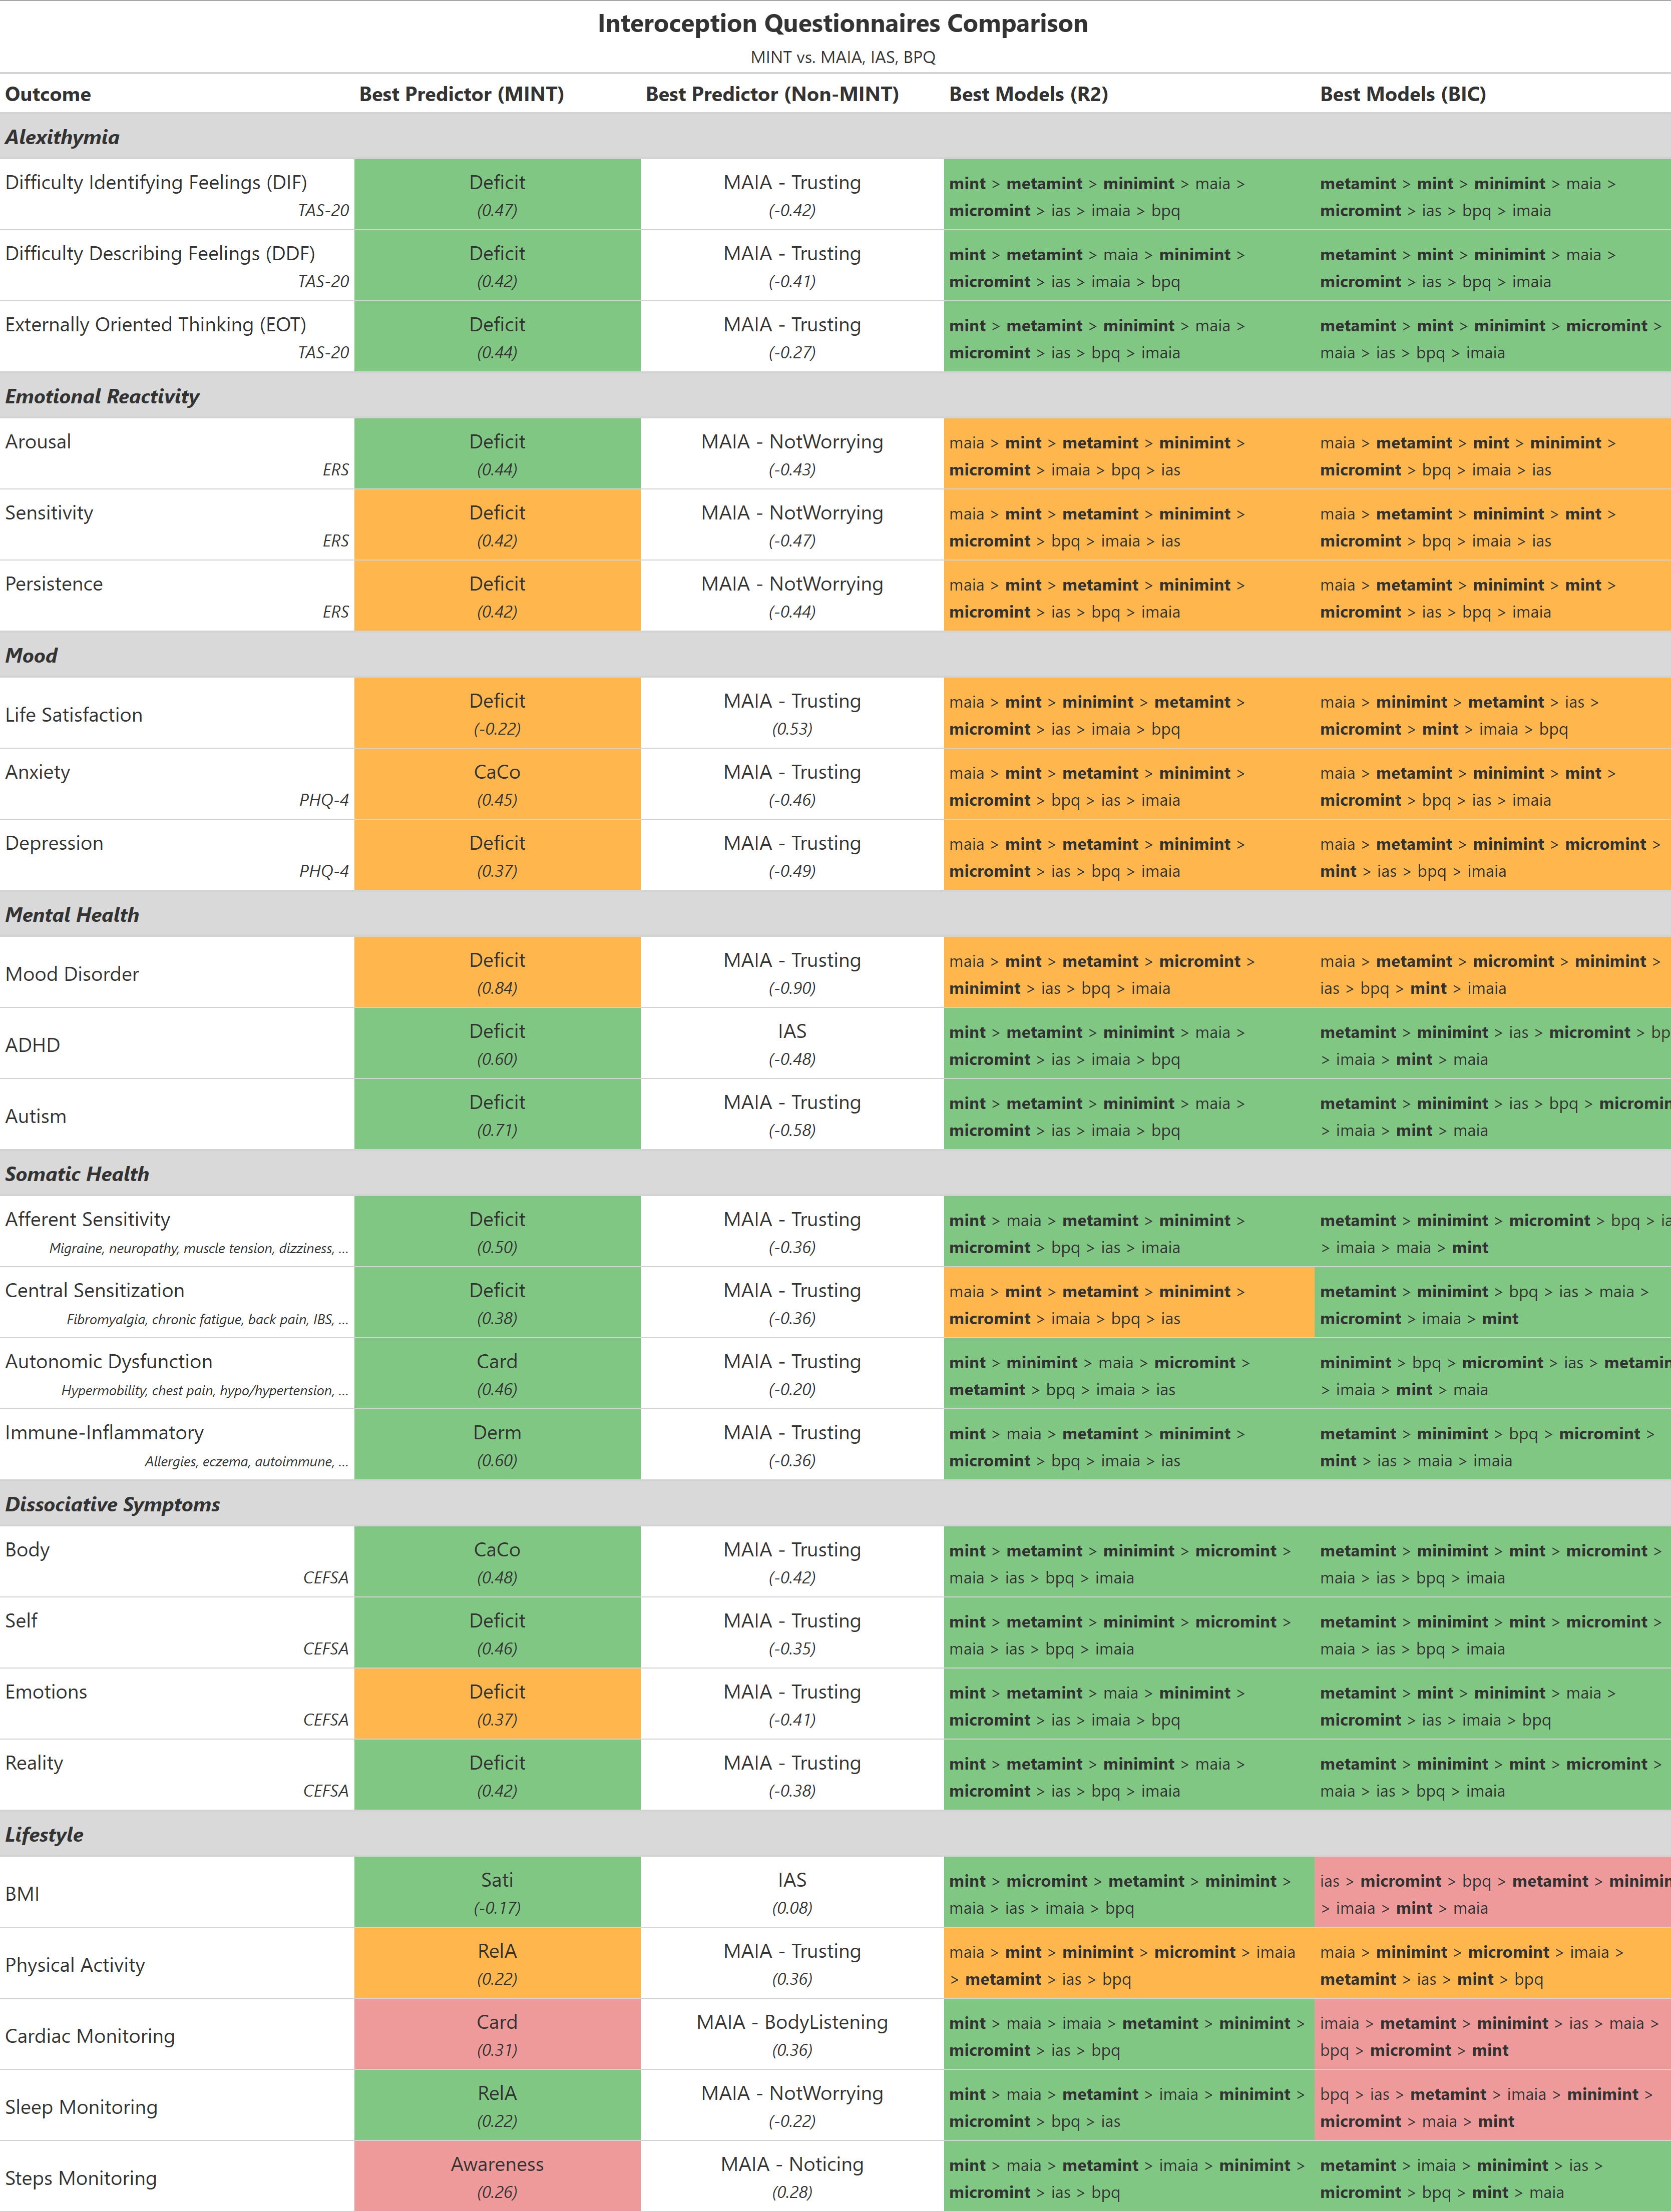
\includegraphics[width=0.82\linewidth,height=\textheight,keepaspectratio]{../study2/analysis/figures/table2.png}
\end{center}

\end{figure*}

Most of the target outcomes measured in the study to assess validity
were best predicted by one of the Mint dimension (see
Figure~\ref{fig-five}). This included Alexithymia (best predicted by
\emph{Deficit}); ERS' Arousal (best predicted by \emph{Deficit});
CEFSA's anomalous experiences of the body (best predicted by
\emph{CaCo}), Self and Reality (best predicted by \emph{Deficit}); ADHD
and Autism (best predicted by \emph{Deficit}), Somatic symptoms (best
predicted by \emph{Deficit}); BMI (best predicted by \emph{Sati}). Most
of the exceptions showed an advantage for MAIA dimensions, in particular
Not-worrying (which best predicted ERS' Sensitivity and Persistence) and
Trusting (which best predicted LS, Depression and Anxiety, CEFSA's
Emotion and Connection, and self-reported physical activity).

Model comparison included 4 variants of the Mint scale, the full
\emph{Mint} (including all lower-level clusters - 33 items), the
\emph{metaMint} (including only the 3 metaclusters based on all items),
the \emph{miniMint} (including the 3 metaclusters computed from 2 of its
most loading triplets - 18 items), and the \emph{microMint} (including
only the most representative dimension of each metacluster - 9 items).
This analysis confirmed the clear advantage for the Mint over the other
interoception scales. The full \emph{Mint} model was typically the best
model based on R2, and the \emph{metaMint} was the best model when
parsimony was taken into account (i.e., based on BIC). Moreover, most of
the instances were the \emph{MAIA} was the best model were explainable
by the inclusion of Trusting, and the interoception-only version
\emph{iMAIA} typically yielded worse performance than the Mint. In many
instances, the \emph{miniMint} yielded reasonable performance, although
the \emph{microMint} was typically less promising.

The predictive performance for the mental health outcomes (see
Figure~\ref{fig-six}) displayed a consistent pattern, with an advantage
for the \emph{MAIA} for depression and anxiety which dropped below the
\emph{Mint} versions for its \emph{iMAIA} variant. The \emph{Mint},
however, displayed a clear advantage for the prediction of autism, ADHD,
and all somatic groups of symptoms (with the exception of Central
Sensitization, which was best predicted by the \emph{MAIA}).

Finally, the importance of heart monitoring (for owners of such
wearable) was best predicted by MAIA's Body listening (\(r = .36\)),
followed the \emph{Card} dimension of the Mint (\(r = .31\)). The
importance of sleep monitoring importance was best predicted by
\emph{RelA} (\(r = .22\)), followed by MAIA's not worrying
(\(r = -.219\)). Daily activity via steps monitoring was best predicted
by MAIA's Noticing (\(r = .28\)), followed by \emph{Awareness}
(\(r = .26\)).

\begin{figure*}[!htbp]

{\caption{{Predictive performance of interoception questionnaires for
various self-reported mental health conditions (mood disorders with
psychopharmacological treatment, ADHD and ASD) and somatic symptoms. The
Receiver Operating Characteristic (ROC) curves are shown for the
logistic regression models for various questionnaires and versions. A
high Area Under the Curve (AUC) indicates a good discriminative power of
the model (i.e., a strong combination of sensitivity and specificity).
The Mint scale (in blue-green) consistently outperformed the other
interoception scales, with the exception of the MAIA which, driven by
its emotion-regulation dimensions (Trusting and Not-worrying), performed
better for mood disorders and central sensitization symptoms. In several
instances, the short versions of the Mint scale (miniMint and microMint)
yielded reasonable performance, still outperforming other
measures.}{\label{fig-six}}}}

\begin{center}
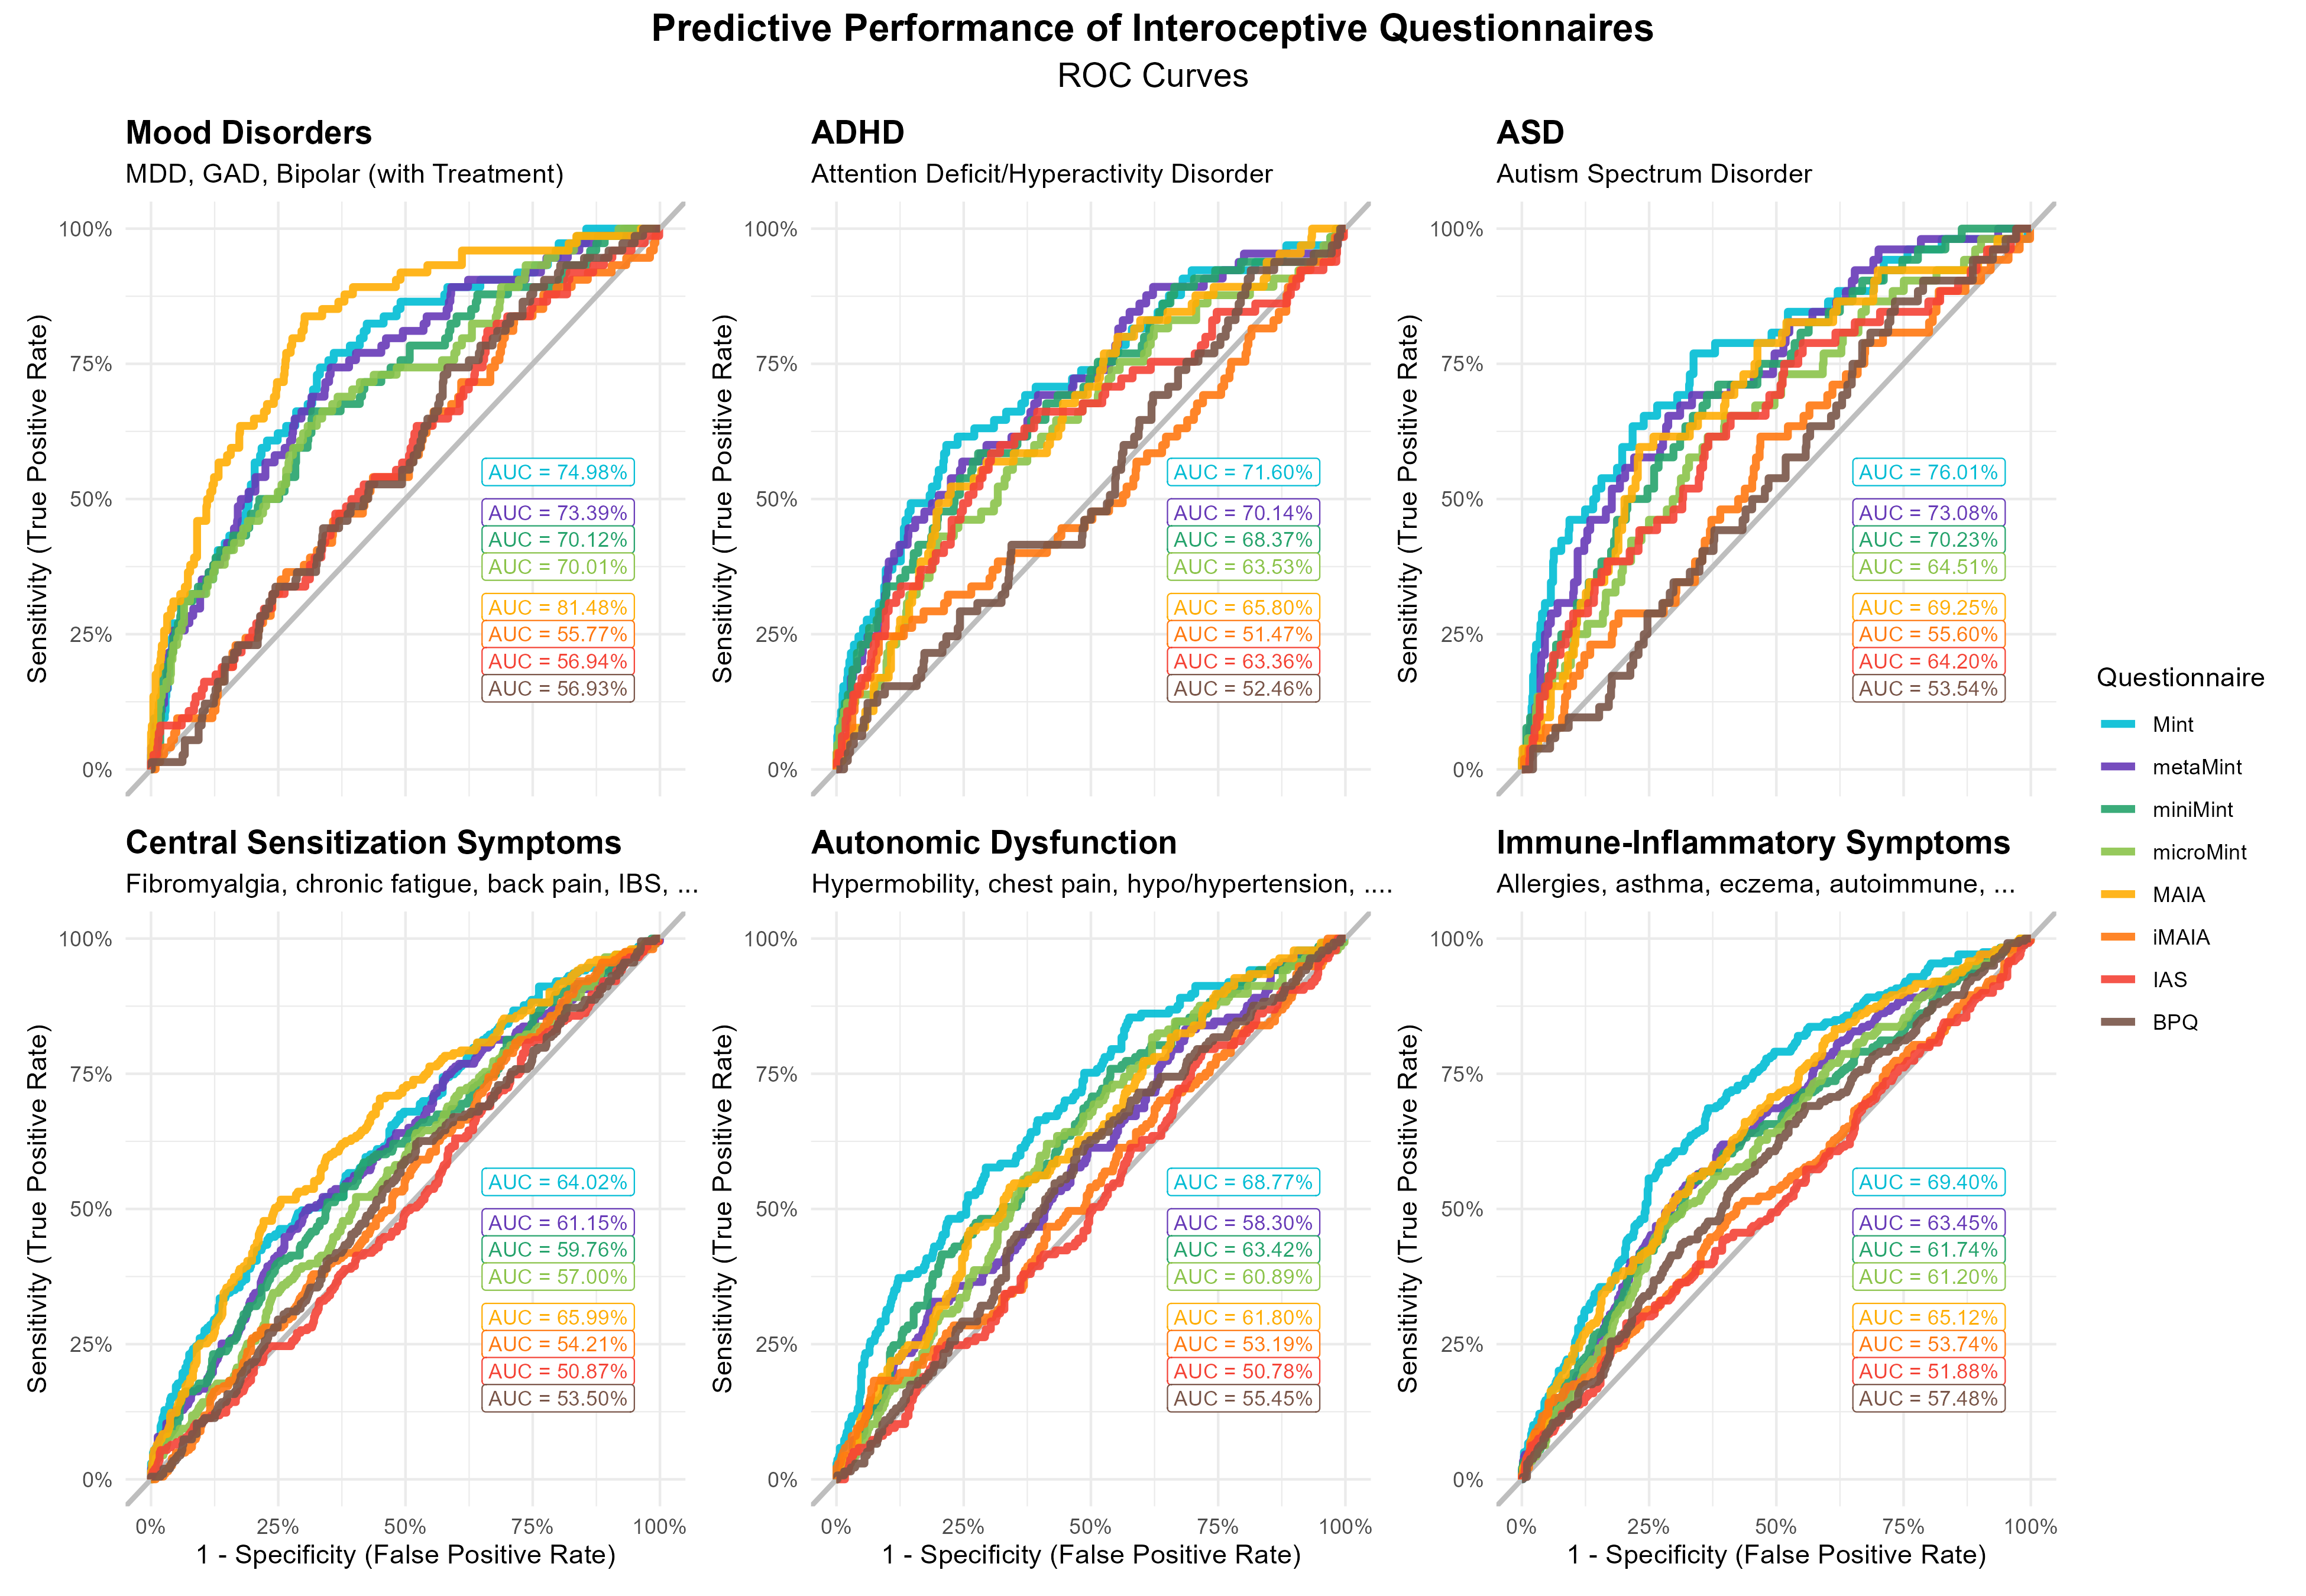
\includegraphics[width=1\linewidth,height=\textheight,keepaspectratio]{../study2/analysis/figures/fig3.png}
\end{center}

\end{figure*}

\subsection{Discussion}\label{discussion-1}

Study 2 sought to formally validate the Mint in a large, independent
sample, a crucial step for establishing the psychometric soundness and
unique contribution of the scale for interoception research. This
involved re-assessing its structure in a new sample and establishing its
convergent and criterion validity against other existing interoception
questionnaires. The analysis led to a final, refined 33-item Mint scale
with a stable and theoretically coherent hierarchical structure, which
demonstrated substantial predictive power across a range of outcomes.

Structure re-validation is an important step following item reduction
since reducing a large item pool can alter the perceived meaning and
relationships between the remaining items. For instance, a questionnaire
with many items suggesting abnormality or pathology might influence the
interpretation of otherwise neutral items. While the original structure
of the Mint was mostly replicated, the re-validation facilitated the
clarification of several higher-order dimensions (e.g., the
``Sensitivity'' metacluster became more clearly defined around core
interoceptive clusters). The final Mint structure, comprising 11 facets
within 3 metaclusters, yielded excellent structural consistency and
stability. The \emph{Olfa} (Olfactory Compensation) cluster had lower
stability within the \emph{Deficit} metacluster, possibly indicative of
a more complex role. For instance, this cluster could be related to
adaptive compensatory processes in some participants and maladaptive
strategies in others. Future studies should further investigate its
place and invariance across different populations and contexts.

The criterion validity analysis revealed a clear and compelling pattern
of results. The Mint scale, particularly its \emph{Deficit} metacluster,
consistently outperformed existing interoceptive scales in predicting
outcomes directly related to alterations in bodily experience and
self-regulation, including alexithymia, dissociative experiences, ADHD,
autism, and various somatic symptoms. The MAIA-2 showed an advantage
over the Mint for predicting outcomes related to general well-being
(e.g., life satisfaction, depression, and anxiety). However, its
predictive superiority was almost entirely driven by dimensions related
to emotion regulation abilities, namely \emph{Trusting} and
\emph{Not-Worrying}, whose inclusion as core interoceptive facets have
been questioned (\citeproc{ref-ferentzi2021examining}{Ferentzi et al.,
2021}). While valuable, the MAIA-2's most predictive subscales appear
less related to core interoceptive processing and more to metacognitive
beliefs about one's body and emotional coping. The Mint, in contrast,
appears to tap more directly into distinct facets of interoceptive
experience, from visceral sensitivity to perceived deficits. Indeed,
when the emotion-regulation dimensions were removed (in the \emph{iMAIA}
version), the MAIA-2's predictive power for well-being outcomes dropped
considerably, often below that of the Mint. Overall, for high-level,
metacognitive aspects of affective state and well-being, the MAIA-2's
emotion regulation facets are highly informative. For outcomes tied more
specifically to bodily processes, clinical conditions characterised by
sensory dysregulation, and nuanced interoceptive experiences, the Mint
offers superior predictive validity and specificity.

\section{General Discussion}\label{general-discussion}

Across two studies, we developed and validated the Multimodal
Interoception Questionnaire (Mint), a new 33-item self-report measure of
interoception. Our approach addressed key limitations of existing
questionnaires by starting with a systematically generated, broad item
pool that explicitly accounted for context and assessed a wide range of
interoceptive modalities. The Mint is a psychometrically robust
instrument with a stable, hierarchical structure comprising three
higher-order metaclusters, namely \emph{Interoceptive Deficit},
\emph{Interoceptive Awareness}, and \emph{Visceroception}, and 11
distinct lower-level facets. Study 2 validated the Mint, demonstrating
that it not only captures variance present in other popular scales
(MAIA-2, BPQ and IAS) but also offers superior predictive power for a
range of clinical and cognitive outcomes, particularly those tied to
altered bodily perception.

A key advantage of the Mint is its potential ability to disentangle core
interoceptive experiences from more general emotion regulation
abilities, an identified problem in interoception research where
findings may be misattributed to ``interoception'' when they are driven
by emotion regulation capacities
(\citeproc{ref-murphy2020testing}{Murphy et al., 2020}). Our findings
show that although the MAIA-2 is a strong predictor of general
well-being, this predictive power is driven by its \emph{Trusting} and
\emph{Not-Worrying} subscales, which heavily tap into emotion regulation
skills and coping strategies. The Mint, in contrast, taps more directly
into interoceptive components, and has excellent predictive power for
conditions where alterations in bodily sensing are a core feature,
including alexithymia, ADHD, autism, and somatic symptoms. Overall, the
Mint provides a more specific measure of self-reported interoceptive
processing across contexts and modalities, offering researchers a
granular and comprehensive tool with which to further understand the
contribution of bodily awareness to human health and disease.

We note several limitations that could serve as the impetus for future
research efforts. First, as a self-report measure, the Mint captures
subjective beliefs about interoceptive abilities, not objective
accuracy. A natural next step will be to establish the extent to which
subjective reports on the Mint correspond to objective interoceptive
performance (e.g., heartbeat tracking tasks, heartbeat evoked
potentials). Second, future research could systematically examine the
usefulness of shorter versions of the Mint, for example, by
investigating the tradeoffs incurred by versions with only the one or
two most central facets per metacluster on psychometric qualities and
predictive power.

While the overall structure of the Mint is stable, some facets warrant
deeper investigation. The \emph{Olfa} (Olfactory Compensation) and
\emph{Derm} (Dermal Hypersensitivity) clusters, for instance, showed
more complex patterns of association. Their placement within the
\emph{Deficit} metacluster is theoretically intriguing since the former
aligns with predictive coding models of pseudo-interoception (or
extero-interoception) where individuals rely on exteroceptive cues (like
odours) to infer internal states
(\citeproc{ref-paulus2010interoception}{Paulus \& Stein, 2010}), while
the latter links visceral and cutaneous sensitivity, possibly reflecting
a general trait of heightened bodily awareness or a shared mechanism of
central sensitization, observed in conditions like chronic pain
(\citeproc{ref-di2016alexithymia}{Di Tella \& Castelli, 2016}). Future
studies should examine the invariance of the Mint's structure across
different populations (e.g., clinical \emph{vs.} non-clinical groups)
and contexts (e.g., heightened arousal \emph{vs.} rest) to clarify the
role of these more nuanced facets. This work could reveal whether the
relevance and pattern of associations are shared or dissociable across
conditions like anxiety disorders, chronic pain, and neurodevelopmental
disorders.

In conclusion, the Mint scale represents a fresh take on interoception
questionnaires and a significant methodological advancement for the
field of interoception research. By providing a validated, structurally
coherent, and nuanced tool, it allows for a more precise assessment of
self-reported interoceptive experiences, paving the way for a deeper
understanding of the multifaceted role of interoception in human
psychology and pathophysiology.

\section{Data Availability}\label{data-availability}

Data, code, and all materials are available at
https://github.com/RealityBending/InteroceptionScale.

\section{Acknowledgements}\label{acknowledgements}

We would like to thank Hugo Critchley for his valuable feedback on the
manuscript. DM would also like to thank Anastasia for the motivation
provided to write this paper.

\section{References}\label{references}

\phantomsection\label{refs}
\begin{CSLReferences}{1}{0}
\bibitem[\citeproctext]{ref-cabrera2018assessing}
Cabrera, A., Kolacz, J., Pailhez, G., Bulbena-Cabre, A., Bulbena, A., \&
Porges, S. W. (2018). Assessing body awareness and autonomic reactivity:
Factor structure and psychometric properties of the body perception
questionnaire-short form (BPQ-SF). \emph{International Journal of
Methods in Psychiatric Research}, \emph{27}(2), e1596.

\bibitem[\citeproctext]{ref-vcernis2024measuring}
Černis, E., Loe, B. S., Lofthouse, K., Waite, P., Molodynski, A.,
Ehlers, A., \& Freeman, D. (2024). Measuring dissociation across
adolescence and adulthood: Developing the short-form {Č}ernis felt sense
of anomaly scale ({Č}EFSA-14). \emph{Behavioural and Cognitive
Psychotherapy}, \emph{52}(2), 163--177.

\bibitem[\citeproctext]{ref-christensen2023unique}
Christensen, A. P., Garrido, L. E., \& Golino, H. (2023). Unique
variable analysis: A network psychometrics method to detect local
dependence. \emph{Multivariate Behavioral Research}, \emph{58}(6),
1165--1182.

\bibitem[\citeproctext]{ref-christensen2021estimating}
Christensen, A. P., \& Golino, H. (2021a). Estimating the stability of
psychological dimensions via bootstrap exploratory graph analysis: A
monte carlo simulation and tutorial. \emph{Psych}, \emph{3}(3),
479--500.

\bibitem[\citeproctext]{ref-christensen2021equivalency}
Christensen, A. P., \& Golino, H. (2021b). On the equivalency of factor
and network loadings. \emph{Behavior Research Methods}, \emph{53}(4),
1563--1580.

\bibitem[\citeproctext]{ref-clifton2021brief}
Clifton, J. D., \& Yaden, D. B. (2021). Brief measures of the four
highest-order primal world beliefs. \emph{Psychological Assessment},
\emph{33}(12), 1267.

\bibitem[\citeproctext]{ref-craig2002how}
Craig, A. D. (2002). How do you feel? Interoception: The sense of the
physiological condition of the body. \emph{Nature Reviews Neuroscience},
\emph{3}(8), 655--666. \url{https://doi.org/10.1038/nrn894}

\bibitem[\citeproctext]{ref-craig2003interoception}
Craig, A. D. (2003). Interoception: The sense of the physiological
condition of the body. \emph{Current Opinion in Neurobiology},
\emph{13}(4), 500--505.

\bibitem[\citeproctext]{ref-critchley2017interoception}
Critchley, H. D., \& Garfinkel, S. N. (2017). Interoception and emotion.
\emph{Current Opinion in Psychology}, \emph{17}, 7--14.
\url{https://doi.org/10.1016/j.copsyc.2017.04.020}

\bibitem[\citeproctext]{ref-crucianelli2023role}
Crucianelli, L., \& Ehrsson, H. H. (2023). The role of the skin in
interoception: A neglected organ? \emph{Perspectives on Psychological
Science}, \emph{18}(1), 224--238.

\bibitem[\citeproctext]{ref-de2015jspsych}
De Leeuw, J. R. (2015). jsPsych: A JavaScript library for creating
behavioral experiments in a web browser. \emph{Behavior Research
Methods}, \emph{47}, 1--12.

\bibitem[\citeproctext]{ref-desmedt2022measures}
Desmedt, O., Heeren, A., Corneille, O., \& Luminet, O. (2022). What do
measures of self-report interoception measure? Insights from a
systematic review, latent factor analysis, and network approach.
\emph{Biological Psychology}, \emph{169}, 108289.

\bibitem[\citeproctext]{ref-desmedt2025discrepancies}
Desmedt, O., Luminet, O., Maurage, P., \& Corneille, O. (2025).
Discrepancies in the definition and measurement of human interoception:
A comprehensive discussion and suggested ways forward.
\emph{Perspectives on Psychological Science}, \emph{20}(1), 76--98.

\bibitem[\citeproctext]{ref-di2016alexithymia}
Di Tella, M., \& Castelli, L. (2016). Alexithymia in chronic pain
disorders. \emph{Current Rheumatology Reports}, \emph{18}(7), 41.

\bibitem[\citeproctext]{ref-ferentzi2021examining}
Ferentzi, E., Olaru, G., Geiger, M., Vig, L., Köteles, F., \& Wilhelm,
O. (2021). Examining the factor structure and validity of the
multidimensional assessment of interoceptive awareness. \emph{Journal of
Personality Assessment}, \emph{103}(5), 675--684.

\bibitem[\citeproctext]{ref-friedman2008sparse}
Friedman, J., Hastie, T., \& Tibshirani, R. (2008). Sparse inverse
covariance estimation with the graphical lasso. \emph{Biostatistics},
\emph{9}(3), 432--441.

\bibitem[\citeproctext]{ref-garfinkel2015knowing}
Garfinkel, S. N., Seth, A. K., Barrett, A. B., Suzuki, K., \& Critchley,
H. D. (2015). Knowing your own heart: Distinguishing interoceptive
accuracy from interoceptive awareness. \emph{Biological Psychology},
\emph{104}, 65--74.
\url{https://doi.org/10.1016/j.biopsycho.2014.11.004}

\bibitem[\citeproctext]{ref-garnefski2006cognitive}
Garnefski, N., \& Kraaij, V. (2006). Cognitive emotion regulation
questionnaire--development of a short 18-item version (CERQ-short).
\emph{Personality and Individual Differences}, \emph{41}(6), 1045--1053.

\bibitem[\citeproctext]{ref-golino2017exploratory}
Golino, H. F., \& Epskamp, S. (2017). Exploratory graph analysis: A new
approach for estimating the number of dimensions in psychological
research. \emph{PloS One}, \emph{12}(6), e0174035.

\bibitem[\citeproctext]{ref-golino2020investigating}
Golino, H., Shi, D., Christensen, A. P., Garrido, L. E., Nieto, M. D.,
Sadana, R., Thiyagarajan, J. A., \& Martinez-Molina, A. (2020).
Investigating the performance of exploratory graph analysis and
traditional techniques to identify the number of latent factors: A
simulation and tutorial. \emph{Psychological Methods}, \emph{25}(3),
292.

\bibitem[\citeproctext]{ref-indahl2018similarity}
Indahl, U. G., Næs, T., \& Liland, K. H. (2018). A similarity index for
comparing coupled matrices. \emph{Journal of Chemometrics},
\emph{32}(10), e3049.

\bibitem[\citeproctext]{ref-jimenez2023dimensionality}
Jiménez, M., Abad, F. J., Garcia-Garzon, E., Golino, H., Christensen, A.
P., \& Garrido, L. E. (2023). Dimensionality assessment in bifactor
structures with multiple general factors: A network psychometrics
approach. \emph{Psychological Methods}.

\bibitem[\citeproctext]{ref-jovanovic2020longer}
Jovanović, V., \& Lazić, M. (2020). Is longer always better? A
comparison of the validity of single-item versus multiple-item measures
of life satisfaction. \emph{Applied Research in Quality of Life},
\emph{15}, 675--692.

\bibitem[\citeproctext]{ref-khalsa2018interoception}
Khalsa, S. S., Adolphs, R., Cameron, O. G., Critchley, H. D., Davenport,
P. W., Feinstein, J. S., \& Zucker, N. (2018). Interoception and mental
health: A roadmap. \emph{Biological Psychiatry: Cognitive Neuroscience
and Neuroimaging}, \emph{3}(6), 501--513.
\url{https://doi.org/10.1016/j.bpsc.2017.12.004}

\bibitem[\citeproctext]{ref-kolacz2018body}
Kolacz, J., Holmes, L., \& Porges, S. W. (2018). Body perception
questionnaire (BPQ) manual. \emph{Traumatic Stress Research Consortium}.

\bibitem[\citeproctext]{ref-kroenke2009ultra}
Kroenke, K., Spitzer, R. L., Williams, J. B., \& Löwe, B. (2009). An
ultra-brief screening scale for anxiety and depression: The PHQ--4.
\emph{Psychosomatics}, \emph{50}(6), 613--621.

\bibitem[\citeproctext]{ref-leising2009toronto}
Leising, D., Grande, T., \& Faber, R. (2009). The toronto alexithymia
scale (TAS-20): A measure of general psychological distress.
\emph{Journal of Research in Personality}, \emph{43}(4), 707--710.

\bibitem[\citeproctext]{ref-ludecke2020extracting}
Lüdecke, D., Ben-Shachar, M. S., Patil, I., \& Makowski, D. (2020).
Extracting, computing and exploring the parameters of statistical models
using r. \emph{Journal of Open Source Software}, \emph{5}(53), 2445.

\bibitem[\citeproctext]{ref-ludecke2021performance}
Lüdecke, D., Ben-Shachar, M. S., Patil, I., Waggoner, P., \& Makowski,
D. (2021). Performance: An r package for assessment, comparison and
testing of statistical models. \emph{Journal of Open Source Software},
\emph{6}(60).

\bibitem[\citeproctext]{ref-ludecke2019insight}
Lüdecke, D., Waggoner, P. D., \& Makowski, D. (2019). Insight: A unified
interface to access information from model objects in r. \emph{Journal
of Open Source Software}, \emph{4}(38), 1412.

\bibitem[\citeproctext]{ref-makowski2025measuring}
Makowski, D., Te, A., Neves, A., \& Chen, S. A. (2025). \emph{Measuring
depression and anxiety with 4 items? Adaptation of the PHQ-4 to increase
its sensitivity to subclinical variability}. PsyArXiv.
\url{https://doi.org/10.31234/osf.io/436np_v2}

\bibitem[\citeproctext]{ref-mayer2011exploratory}
Mayer, C.-D., Lorent, J., \& Horgan, G. W. (2011). Exploratory analysis
of multiple omics datasets using the adjusted RV coefficient.
\emph{Statistical Applications in Genetics \& Molecular Biology},
\emph{10}(1).

\bibitem[\citeproctext]{ref-mehling2018multidimensional}
Mehling, W. E., Acree, M., Stewart, A., Silas, J., \& Jones, A. (2018).
The multidimensional assessment of interoceptive awareness, version 2
(MAIA-2). \emph{PloS One}, \emph{13}(12), e0208034.

\bibitem[\citeproctext]{ref-murphy2020testing}
Murphy, J., Brewer, R., Plans, D., Khalsa, S. S., Catmur, C., \& Bird,
G. (2020). Testing the independence of self-reported interoceptive
accuracy and attention. \emph{Quarterly Journal of Experimental
Psychology}, \emph{73}(1), 115--133.

\bibitem[\citeproctext]{ref-murphy2018classifying}
Murphy, J., Catmur, C., \& Bird, G. (2018). Classifying individual
differences in interoception: Implications for the measurement of
interoceptive accuracy. \emph{Psychonomic Bulletin \& Review},
\emph{25}(4), 1424--1431.
\url{https://doi.org/10.3758/s13423-017-1339-z}

\bibitem[\citeproctext]{ref-paulus2010interoception}
Paulus, M. P., \& Stein, M. B. (2010). Interoception in anxiety and
depression. \emph{Brain Structure and Function}, \emph{214}(5),
451--463.

\bibitem[\citeproctext]{ref-Rcoreteam}
R Core Team. (2025). \emph{R: A language and environment for statistical
computing}. R Foundation for Statistical Computing.
\url{https://www.R-project.org/}

\bibitem[\citeproctext]{ref-sibson1978studies}
Sibson, R. (1978). Studies in the robustness of multidimensional
scaling: Procrustes statistics. \emph{Journal of the Royal Statistical
Society: Series B (Methodological)}, \emph{40}(2), 234--238.

\bibitem[\citeproctext]{ref-theriault2024check}
Thériault, R., Ben-Shachar, M. S., Patil, I., Lüdecke, D., Wiernik, B.
M., \& Makowski, D. (2024). Check your outliers! An introduction to
identifying statistical outliers in r with easystats. \emph{Behavior
Research Methods}, \emph{56}(4), 4162--4172.

\bibitem[\citeproctext]{ref-traag2019louvain}
Traag, V. A., Waltman, L., \& Van Eck, N. J. (2019). From louvain to
leiden: Guaranteeing well-connected communities. \emph{Scientific
Reports}, \emph{9}(1), 1--12.

\bibitem[\citeproctext]{ref-veilleux2024development}
Veilleux, J. C., Schreiber, R. E., Warner, E. A., \& Brott, K. H.
(2024). Development and validation of a brief version of the emotion
reactivity scale: The b-ERS. \emph{Current Psychology}, \emph{43}(14),
12586--12600.

\bibitem[\citeproctext]{ref-vig2022questionnaires}
Vig, L., Köteles, F., \& Ferentzi, E. (2022). Questionnaires of
interoception do not assess the same construct. \emph{PLoS One},
\emph{17}(8), e0273299.

\bibitem[\citeproctext]{ref-zamariola2018interoceptive}
Zamariola, G., Maurage, P., Luminet, O., \& Corneille, O. (2018).
Interoceptive accuracy scores from the heartbeat counting task are
problematic: Evidence from simple bivariate correlations.
\emph{Biological Psychology}, \emph{137}, 12--17.

\end{CSLReferences}






\end{document}
